%! TEX program = xelatex
\documentclass{article}
\usepackage[UTF8]{ctex}
\usepackage{geometry}
\geometry{left=2cm,right=2cm,top=2cm,bottom=2cm}
\usepackage[hidelinks]{hyperref}
\usepackage{amsmath}
\usepackage{lmodern}
\usepackage{footnote}
\usepackage{graphicx}
\usepackage{float}
\usepackage{placeins}
\usepackage{xparse}
\usepackage{listings}
\usepackage{fontspec}
\usepackage{color}
\usepackage{xcolor}
\usepackage{fancyhdr}
\usepackage{comment}
\usepackage{textcomp}
\usepackage{titlesec}
\usepackage{titletoc}
\usepackage{longtable}
\usepackage{enumitem}
\usepackage{booktabs}
\usepackage{float}
\usepackage[sort]{natbib}
\usepackage{subfigure}
\usepackage{tabularx}
\usepackage{wrapfig}
\usepackage{multirow}
\usepackage{textcomp}
\graphicspath{{res/}}

\fancypagestyle{plain}{
	\pagestyle{fancy}      %改变章节首页页眉
}

%\pagestyle{fancy}
%\lhead{\kaishu~课程论文~}
%\rhead{\kaishu~2020 年 11 月 5 日}
\cfoot{\thepage}


\setmonofont[
    Contextuals={Alternate},
    ItalicFont = Fira Code      % to avoid font warning
]{Fira Code}
\definecolor{codegreen}{rgb}{0,0.6,0}
\definecolor{codegray}{rgb}{0.5,0.5,0.5}
\definecolor{codepurple}{rgb}{0.58,0,0.82}
\definecolor{backcolour}{rgb}{0.95,0.95,0.92}

\lstset{
	backgroundcolor=\color{backcolour},   
	commentstyle=\color{codegreen},
	keywordstyle=\color{magenta},
	numberstyle=\tiny\color{codegray},
	stringstyle=\color{codepurple},
	basicstyle=\normalsize,
	breakatwhitespace=false,         
	breaklines=true,                 
	captionpos=b,                    
	keepspaces=true,                 
	numbers=left,                    
	numbersep=10pt,                  
	showspaces=false,                
	showstringspaces=false,
	showtabs=false, 
    %escapebegin=\begin{CJK*}{GBK}{hei},escapeend=\end{CJK*},
	tabsize=4
}

\NewDocumentCommand{\inputCode}{ O{matlab} m }{
	{
		\setmainfont{FiraCode Nerd Font}[
		ItalicFont  = FiraCode Nerd Font
		]
		\lstinputlisting[
		basicstyle=\codeF,
		language=#1,
		tabsize=4,
		showstringspaces=false,
		breaklines=true,
		frame=shadowbox,
		framexleftmargin=10mm,
		rulesepcolor=\color{black},
		basicstyle=\large\monaco,
		numbers=left,
		xleftmargin=3em,
		]{#2}
	}
}
\renewcommand{\contentsname}{目录}
\titlecontents{section}[0em]{\songti\zihao{-4}}{\thecontentslabel\ }{}
{\hspace{.5em}\titlerule*[4pt]{$\cdot$}\contentspage}
\titlecontents{subsection}[2em]{\vspace{0.1\baselineskip}\songti\zihao{-4}}{\thecontentslabel\ }{}
{\hspace{.5em}\titlerule*[4pt]{$\cdot$}\contentspage}
\titlecontents{subsubsection}[4em]{\vspace{0.1\baselineskip}\songti\zihao{-4}}{\thecontentslabel\ }{}
{\hspace{.5em}\titlerule*[4pt]{$\cdot$}\contentspage}

\newcommand{\upcite}[1]{\textsuperscript{\textsuperscript{\cite{#1}}}}
\title{\LARGE 基于平衡状态的数据中心散热分析}
%\author{光电1902 郑文斌}
\begin{document}
	%\maketitle
	\begin{table}[H]
		\centering
		\begin{tabular}{cc}
			\toprule[1.5pt]
			队伍编号  & XXXXX \\
			\midrule
			题目    & C \\
			\bottomrule[1.5pt]
		\end{tabular}%
	\end{table}%
	\begin{center}
	\LARGE 基于平衡状态的数据中心散热分析
    \end{center}
	\large

	\textbf{摘要}  \quad 	对于海底数据中心,如何在有限的体积内存放更多的服务器且保证服务器工作过程中向海水中正常快速的散热是一项非常有挑战性的问题。本文的目标是海底数据中心的优化设计,给微软,谷歌,华为等公司的海底数据中心的外壳散热提供设计方案。
	
	本文首先研究了\textbf{纯体积限制}下的最大服务器数量,为\textbf{609}台(局部最优,可能有更大值),作为服务器数量的上限。其次建立了圆柱体内部空气与外壳的热传导模型,外壳与海水的自然对流和强制对流模型。发现对于给定的中心温度和其他相关值,体系存在\textbf{负反馈稳定状态},即\textbf{圆柱体表面温度存在唯一值},于是转化为对稳定状态量的求解。通过努塞尔数建立表面温度与海水温度差和服务器容纳量之间的关系,最后求解得到最大服务器量。
	
	对于问题一,在自然对流和强制对流情况下,遍历传热系数$h$的可能值,使用逼近搜索的算法寻找平衡状态量,得到表面温度值,进而计算得自然对流和强制对流情况下的表面温度为$36 ^\circ C ,24 ^\circ C$,最大服务器数量分别为\textbf{282,572}台。
	
	对于问题二,首先长方体外形结构不抗压,因此应该设计成圆柱体或者球体结构;然后我们考虑了翅片结构和格栅结构,它们通过增大表面积提高服务器数量。
	
	对于问题三,对附件中材料数据进行预处理,形成6个材料类:铝合金、铜和铜合金、镍合金、铁类、钛和钛合金、不锈钢。同一类的材料性质相近,使用取均值的方式进行汇总。用元素价格表征成本量,用弹性模量、屈服强度、拉伸强度表征抗压能力,用海水电位表征抗腐蚀能力,建立\textbf{3准则6方案的层次分析法模型},得到铁和钛合金的得分最高,分别为\textbf{0.22,0.21},因此可以\textbf{以铁为主要材料},以钛合金为涂层,达到降低成本同时抗压抗腐蚀能力。
	
	对于问题四,潮汐和季节的变化主要影响海水温度、海水流速以及来流角度,对潮汐和季节的研究转化为海水温度、海水流速以及来流角度的变化对散热及服务器数量的影响。设置2次循环遍历,得到服务器数量与温度呈现\textbf{负的一次函数关系},与海水流速呈现\textbf{对数关系}。当海水温度由$0$升高到$25^\circ C$,服务器数量(自然对流状态下)由385台降低为265台;服务器数量随海水流速的上升而上升,当流速大于0.5m/s,可容纳的服务器数量上升缓慢。当海水流向平行于圆柱体轴线时,服务器数量降低为250台。
	
	最后,分析了模型的优缺点,并作了建议信。
	\\
	\par
	\noindent\textbf{关键词:\quad 牛顿冷却定律 \quad 自然和强制对流\quad 负反馈平衡状态 \quad 遍历搜索逼近法 \quad 层次分析法}
	\newpage
	
	\tableofcontents
	\thispagestyle{empty}
	\newpage
	\setcounter{page}{1}
	\section{问题重述}
	对于海底数据中心,如何在有限的体积内存放更多的服务器且保证服务器工作过程中向海水中正常快速的散热是一项非常有挑战性的问题。现在各位参赛队员将参与到海底数据中心的优化设计,解决如下问题,并给微软,谷歌,华为等公司的海底数据中心的外壳散热提供设计方案。
	
	问题1:固体在液体中的冷却的方式主要是对流传热,对流传热可分为自然对流和强制对流。假定数据中心集装箱的尺寸为直径1m,长12m的圆柱形,悬空放置(圆柱形轴线与海平面平行)在中国南海温度为20 摄氏度的海域深度,其中单个1U 服务器的产热为500W(正常工作温度不能超过80 摄氏度),1U 服务器机箱的高度为44.45 毫米,宽度为482.6 毫米,长度为525毫米,请评估单个集装箱外壳中最多可以放多少个服务器(仅考虑服务器的散热需求)。
	
	问题2:假定集装箱外壳最大尺寸不超过1m×1m×12m,结合第一问的分析,如何设计集装箱外壳的结构(如在圆柱体,长方体等上考虑翅片结构),可以实现最大化的散热效果,即存放更多的服务器。
	
	问题3:较深的海水具有较低的温度,能取得更好的散热效果,同时增大的压力会对集装箱外壳的耐压能力提出更高的要求;值得注意的是海水本身是一种强的腐蚀介质,直接与海水接触的各种金属结构物都不可避免地受到海水的腐蚀。请在问题2 的基础上进一步选择合适的材料和海底深度进行优化设计,进一步提高散热效果,并尽可能降低成本,提高使用年限。
	
	问题4:潮汐和季节会改变局部水位和温度,并带来暂时性的海水流动,可能对数据中心的散热带来一定影响。请考虑潮汐和季节变化等因素对海底数据中心集装箱散热效果的影响。
	
	问题5:竞赛组委会希望大家可以根据自己的分析结果写一封建议信给相关公司的海底数据中心散热设计部门。
	
	\section{问题分析}
	求解圆柱体最大服务器容纳量的问题,实际上可以归结为综合考虑各种传热方式,建立热传导和热对流模型,其中圆柱体内部主要为热传导,圆柱体外部主要为热对流。然后建立圆柱体内外不同模型的联系。对于给定的足够参数,存在唯一的平衡状态,我们的目标就是建立相关算法求解稳定状态。
	
	首先我们需要了解自然对流换热和强制对流换热的适用范围。
	
	1. 自然对流换热:参与换热的流体由于各部分温度不均匀而形成密度差,从而在重力场或其他力场中产生浮升力所引起的对流换热现象。
	
	2、强制对流换热:液体或气体在外力影响下所发生的对流,即海水本身在流动,存在初始速度。
	
	对于问题1,考虑“散热效果”和“存放的服务器数量”2个因素,首先纯按体积限制计算最大服务器容纳量,作为服务器数量的上限。然后考虑自然对流和强制对流情况下的散热模型,计算只考虑散热情况下的服务器数量。
	
	对于问题3,需要寻找最佳材料,附件中的材料太多,应该首先进行提取,分类,归一等等,建立多因素评价模型;
	
	对于问题4,潮汐和季节会改变局部水位和温度,并带来暂时性的海水流动,可能对数据中心的散热带来一定影响。温度变化主要是由于季节改交造成的,此因素需要结合问题1进行
	分析,在问题1的模型上加入温度变化这个因子;海水流动的原因与潮汐和季节改变都有关,海水流动会造成流速加快,会让海水降温更快,即考虑强制对流情况下海水流速对散热的影响。
	
	
	
	\section{模型假设}
		\begin{itemize}
			\item 服务器主要集中分布在圆柱体轴线上,圆柱体轴线上温度最高,为最大允许温度$80^\circ C$;
			\item 建立传热模型时圆柱体看作无限长圆管,两圆形底面不代入计算;
			
			\item 空气的传热系数为$20-100 W/(m^{2} K)$,由于圆柱体内温度较高,传热系数取最大值$100 K/(m^{2 } K)$;
			\item 计算强制对流情况下的服务器数量时,不作其他说明,默认海水流速为$1 m/s$;
		\end{itemize}	
	
	\section{符号说明}
	\begin{table}[H]
	\centering
	\caption{符号表}
	\begin{tabularx}{0.9\textwidth}{@{}c *2{>{\centering\arraybackslash}X}@{}}
		\toprule[1.5pt]
		变量    & 说明    & 量纲 \\
		\midrule
		N     & 服务器最大数量 & 台 \\
		P     & 单台服务器产热功率 & W \\
		S     & 圆柱体表面积 & $m^2$ \\
		To    & 圆柱体中心温度 & $^\circ C$ \\
		Ts    & 圆柱体表面温度 & $^\circ C$ \\
		Tr    & 海水温度  & $^\circ C$ \\
		$T_m$ & 特征温度,即海水与外壳的平均温度  &   $^\circ C$ \\ 
		$h,h_2$  & 海水与圆柱体外壳之间的传热系数 & $W/(m^2 K)$ \\
		$h_1$    & 圆柱体内部空气与内壁之间传热系数 & $W/(m^2 K)$ \\
		k     & 导热系数  & $W/(m K)$ \\
		L     & 特征长度  & m  \\
		Nu    & 努塞尔数,表示对流换热强烈程度 & - \\
		Re,Pr,Gr,Ra & 雷诺数,普朗特数,格拉晓夫数,瑞利数 & - \\
		g     & 重力加速度 & $m/s^2$ \\
		$\beta$  & 热膨胀系数 & - \\
		$\nu$    & 运动黏度  & $Pa \cdot s$ \\
		u     & 海水流速  & m/s \\
		\bottomrule[1.5pt]
	\end{tabularx}%
	\label{}%
\end{table}%
	
	\section{相关物理模型的建立}
	

	
    \subsection{箱体满载服务器量}
    考虑在圆柱体箱在放置长方体服务器的最大数量,以下是服务器排放的示意图:
    \begin{figure}[H]
    	\centering
    	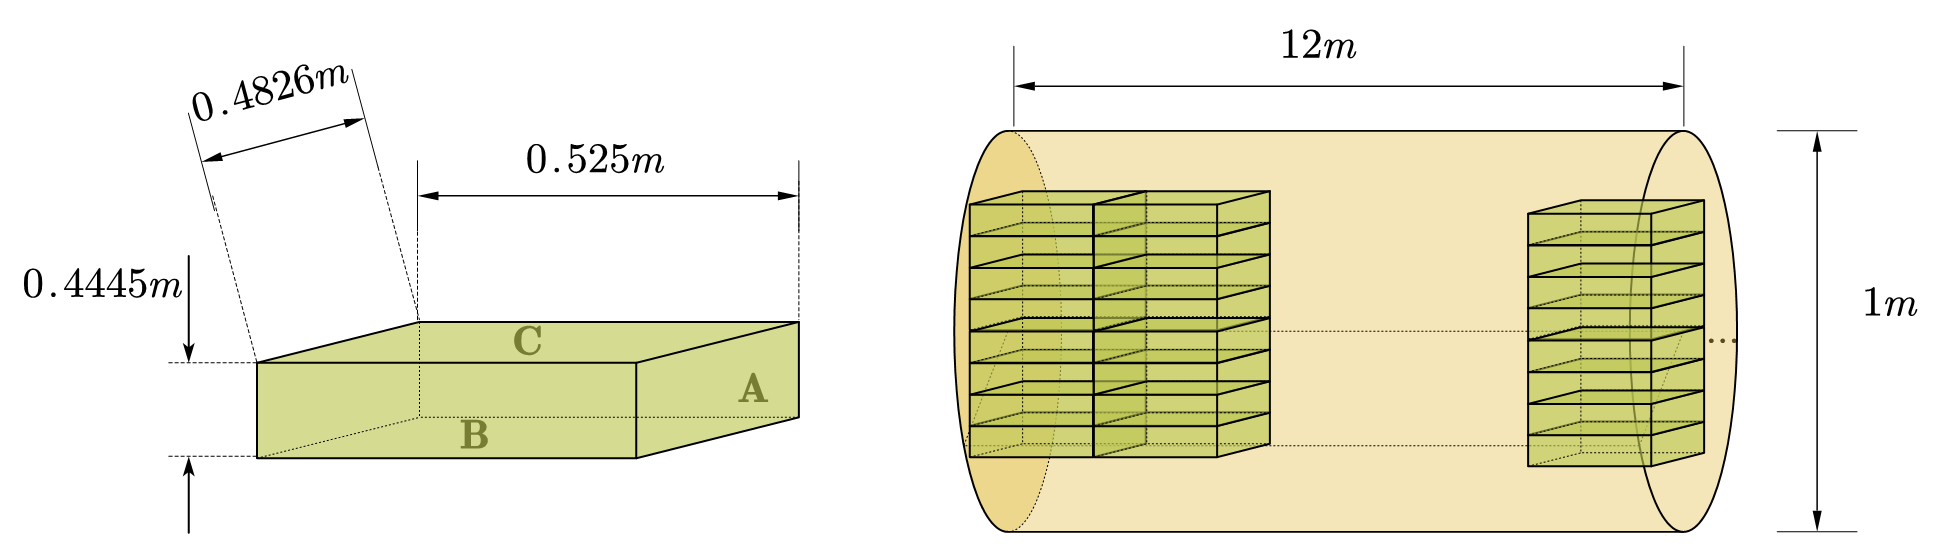
\includegraphics[width=0.9\textwidth]{img/摆放.png}
    	\caption{服务器排放的示意图}\label{fig:baifang}
    \end{figure}
   其中长方体的3个面的编号如下表:
   \begin{table}[H]
   	\centering
   	\begin{tabularx}{0.9\textwidth}{@{}c *3{>{\centering\arraybackslash}X}@{}}
   		\toprule[1.5pt]
   		编号    & A     & B     & C \\
   		\midrule
   		边长 $\times$ 边长 & $0.04445 \times 0.4826$ & $0.04445 \times 0.525$ & $0.525 \times 0.4826$ \\
   		\bottomrule[1.5pt]
   	\end{tabularx}%
   	\label{tab:}%
   \end{table}%
   
   目标就是在有限的体积($\pi r^2 \times 12m$)内存放更多的服务器,我们需要根据圆柱体半径、高与小长方形的长、宽、高的比例关系来确定小长方形在圆柱体是如何摆放,实际上是一个排列组合问题。
   
   首先考虑紧贴圆柱体底面的不同大小的面A、B、C,如图:
   \begin{figure}[H]
   	\centering
   	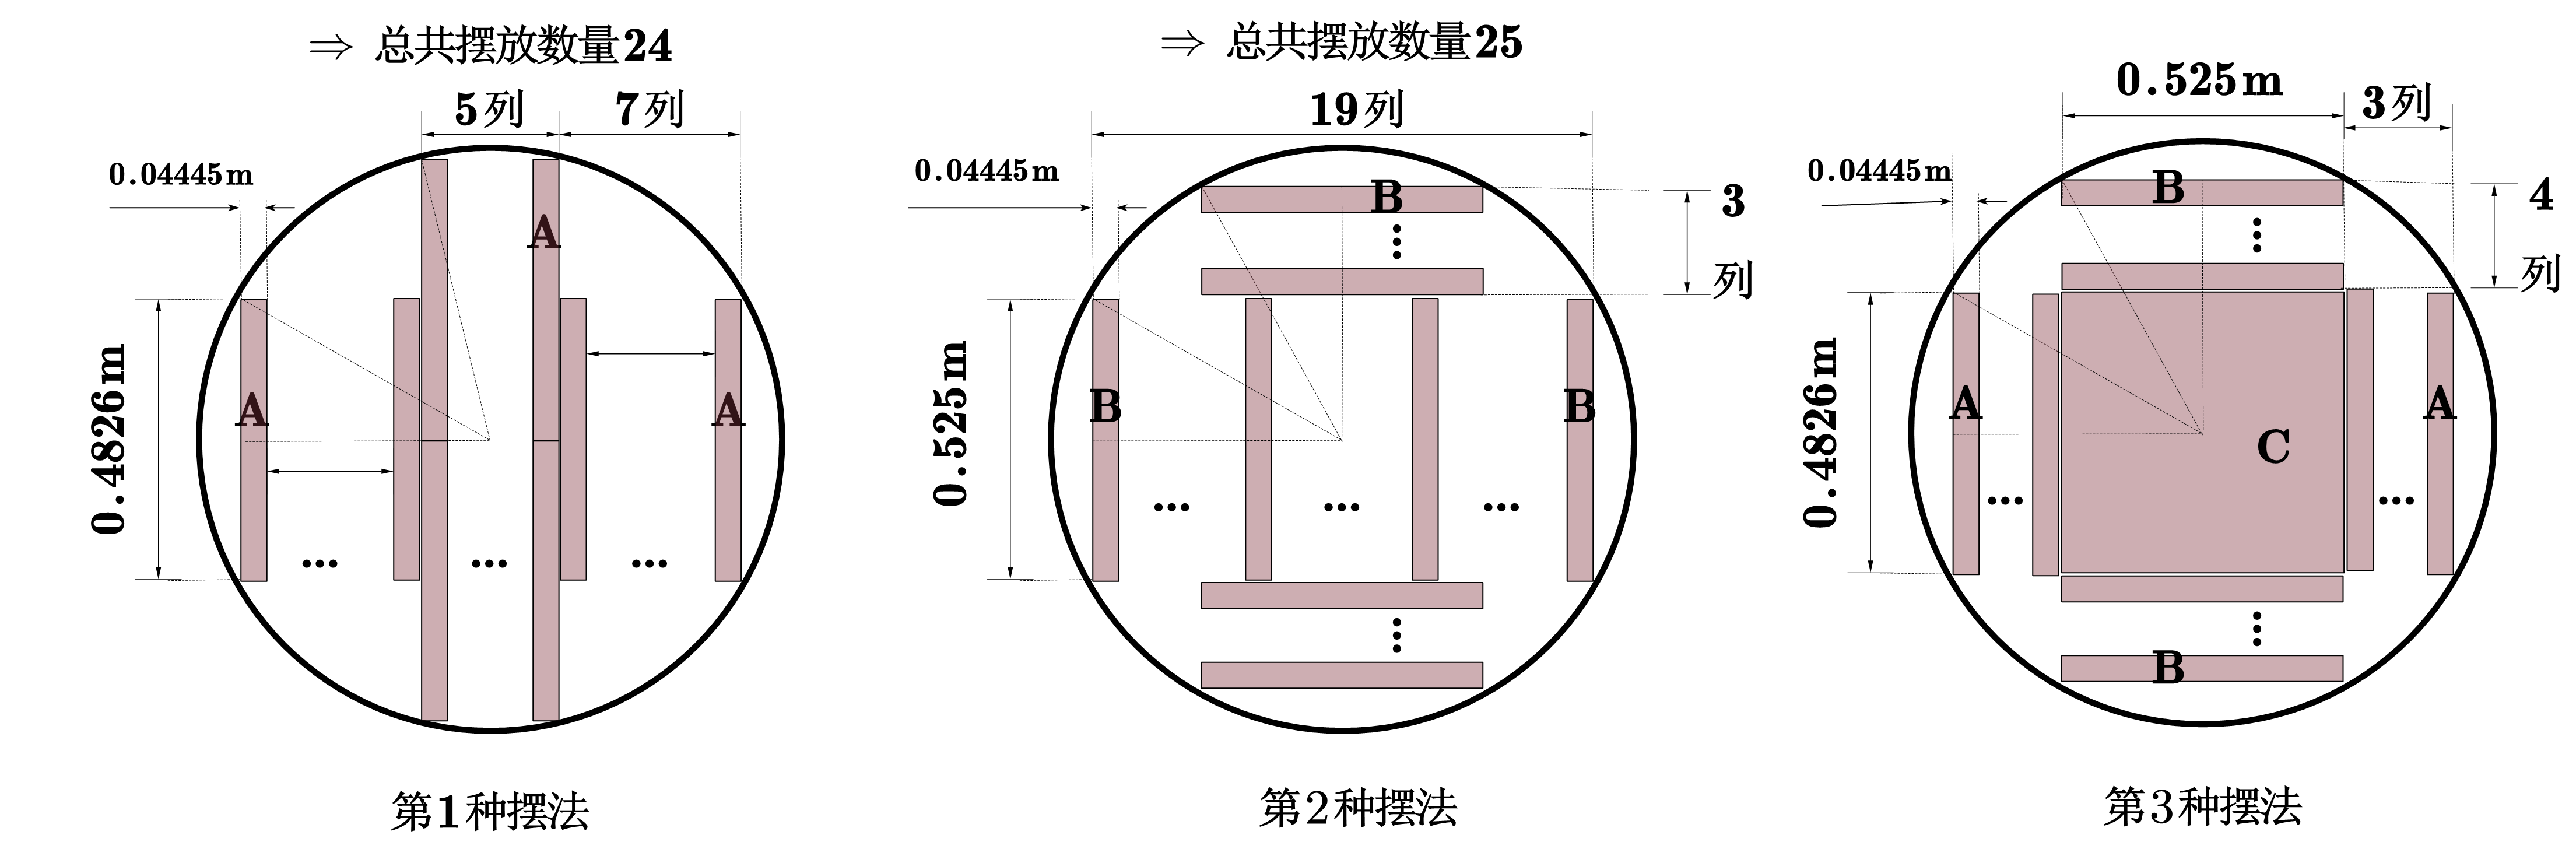
\includegraphics[width=1.0\textwidth]{img/所有摆法.png}
   	\caption{不同底面的摆放方式}\label{fig:suoyoubaifang}
   \end{figure}
   总摆放数量N:
   
   \begin{equation}
   N= d \times layer+\max \left( floor \left(\frac{12000- h \times layer }{l}\right),  floor \left(\frac{12000- h \times layer }{w}\right)\right)
   \label{baifangshuliang}
   \end{equation}
   
   
   其中$d$为底面摆放数量,
   $$
   \ layer = floor \left(\frac{12000}{h}\right)
   $$
   为摆放层数。
   
   由公式\eqref{baifangshuliang}计算3种摆放方式的总摆放数量N,对于摆法3,由于B、C同时作为底面,计算应做相应的调整;计算结果如下:
   \begin{table}[htbp]
   	\centering
   	\caption{3种方案对应的最大摆放数量}
   	\begin{tabularx}{0.9\textwidth}{@{}c *3{>{\centering\arraybackslash}X}@{}}
   		\toprule[1.5pt]
   		摆法方案  & 1     & 2     & 3 \\
   		\midrule
   		描述    & A面作为底面 & B面作为底面 &B,C面作为底面 \\
   		最大摆放数量 & 538   & 609   & 593 \\
	    \bottomrule[1.5pt]   		
   	\end{tabularx}%
   	\label{tab:shujv}%
   \end{table}%

   从上表得出,在只考虑体积影响因素的前提下,箱体满载服务器量为609台(局部最优解,可能还有其他情况大于此值)。
   
   \subsection{牛顿冷却定律和努塞尔数}
   定义热流密度q:
   $$q = \frac{NP}{S}$$
   其中N为服务器数量,P为单个服务器产热功率,S为圆柱体表面积。
   
   牛顿冷却定律表述为
   \begin{equation}
   q = h(T_s-T_r)
   \label{niudun}
   \end{equation}
   其中,$T_s$为圆柱体表面温度,$T_r$为海水温度,$h$为传热系数,S=$12.5\pi$ 为圆柱体表面积。
   由此可导出服务器数量公式:
   \begin{equation}
   N= \frac{h(T_s-T_r)S}{P}
   \label{N}
   \end{equation}
   
   努塞尔数$ N_u$ 是边界上的对流换热与传导换热的比值。对流热流与传导热流相互平行,并与边界表面法线平行,在简单情况下均垂直于平均流体流动。
   \begin{equation}
   {Nu}_{L}=\frac{\text { 对流传热 }}{\text { 传导传热 }}=\frac{h}{k / L}=\frac{h L}{k}
   \label{Nu}
   \end{equation}
   其中$h$是流体的对流传热系数,$L$是特征长度,$k$是流体的热导率。
   
   联立公式\eqref{N}\eqref{Nu}得
   \begin{equation}
   N=\frac{Nu k(T_s-T_r)S}{L P}
   \label{N2}
   \end{equation}
   通常,对于自由对流,平均Nusselt数表示为Rayleigh数和Prandtl数的函数,写为:
	\begin{equation}
	{Nu}=f(\mathrm{Ra}, \mathrm{Pr})
	\end{equation}
   否则,对于强制对流,Nusselt数通常是雷诺数和Prandtl数的函数,或者
   \begin{equation}
   {Nu}=f(\operatorname{Re}, \operatorname{Pr})
   \end{equation}
   可以使用以上述形式表示Nusselt数的各种几何形状的经验相关性。
   
   \noindent 雷诺数(Re)为表征流体惯性力与粘性力的相对大小,通常根据雷诺数判断流态。
	\begin{equation}
	R e=\frac{u L}{\nu}
	\end{equation}
   普朗特数(Pr)是流体的物性特征数,表征流体动量扩散能力与热量扩散能力的相对大小。
   \begin{equation}
   Pr=\frac{\nu}{a}
   \end{equation}
   格拉晓夫数(Gr)为一无量纲的标量,常用在流体力学及热传导中。格拉晓夫数可以视为流体浮力与粘性力的比值
   \begin{equation}
   \mathrm{Gr}=\frac{g \beta\left(T_{s}-T_{r}\right) L^{3}}{\nu^{2}}
   \end{equation}
   Gr数与Pr数之积称为拉格利数,记为Ra:
   \begin{equation}
   R a=G r Pr=\frac{g \beta\left(T_{s}-T_{r}\right) L^{3}}{\nu^{2}} Pr
   \label{Ra}
   \end{equation}
   
   \subsection{自然对流模型(海水静止)}   
   流体受壁面加热或冷却而引起的自然对流换热 与流体在壁面附近的由温度差异所形成的浮升力有关。不均匀的温度场造成了不均匀的密度场,由此产生的浮升力成为运动的动力。
   \begin{wrapfigure}{r}{4cm}
   	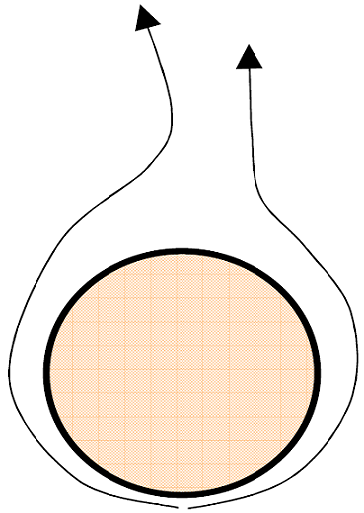
\includegraphics[width=3cm]{img/自然对流.png}
   \end{wrapfigure}
   一般情况下,不均匀温度场仅发生在靠近换热壁面的薄层之内。在贴壁处,流体温度等于壁面壁面温度$T_s$,在离开壁面的方向上逐步降低至周围环境温度。 
  
   当海水无外力扰动的情况下,热圆柱体与冷海水之间的热交换形式主要为自然对流.
   \par
   \par
   
   \begin{equation}
   N u=c(G r \operatorname{Pr})^{n}
   \end{equation}
   其中定性温度为:
   \begin{equation}
   T_{m}=\left(t_{s}+t_{r}\right) / 2
   \end{equation}
   对于水平放置圆管(圆柱体),流动状态为层流时,$c=0.53,n=0.25$,适用范围(GrPr)为$10^{5} \sim 10^{9}$
   
   另外Churchill 和Chu 提出的适用范围大的计算公式:
   \begin{equation}
   Nu=\left\{0.6+\frac{0.387 R a^{1 / 6}}{\left[1+(0.559 / \operatorname{Pr})^{9 / 16}\right]^{8 / 27}}\right\}^{2}
   \label{Nu1}
   \end{equation}
   式中准则的特征尺寸为圆柱体外直径d、定性温度为膜温度$T_m$、适用范围是
   GrPr=$10^5 \sim 10^{12}$
   \subsection{强制对流模型(海水横掠单管)}
   横掠单管:流体沿着垂直于管子轴线的方向流过管子表面。如下是流体横掠单管的示意图:
   \begin{figure}[H]
   	\centering
   	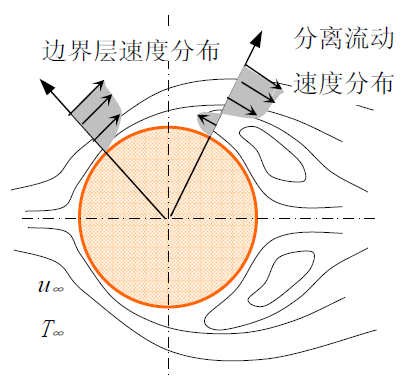
\includegraphics[width=0.3\textwidth]{img/示意图.png}
   	\caption{流体横掠单管的示意图}\label{fig:shiyitu}
   \end{figure}
   流体外掠(横向掠过)单根圆管换热的经验关系式:
   \begin{equation}
   Nu=C * \operatorname{Re}^{n} * \operatorname{Pr}^{1 / 3}
   \end{equation}
   流体绕流圆柱体的平均换热系数也可采用以下朱考斯卡斯经验公式计算:
   \begin{equation}
   N u=\frac{{h} d}{k}=C* \operatorname{Re}^{n }* \operatorname{Pr}_{r}^{0.37} *\left(\frac{\operatorname{Pr}_{r}}{\operatorname{Pr}_{s}}\right)^{0.25}
   \label{Nu2}
   \end{equation}
   其中,特征流速为流体最小截面处的最大流速$v$,特征尺寸为圆柱体外直径d;定性温度除$Pr_s$按壁面温$T_s$取值之外,其余皆用流体的平均温度$T_r$
   
   $\left(\frac{\operatorname{Pr}_{r}}{\operatorname{Pr}_{s}}\right)^{0.25}$是考虑在选用$T_r$为定性温度时,热流方向不同会对换热性能产生影响的一个修正系数.
   
   流体绕流单圆柱体时的常数C、n 数值表如下:
   $$
   \begin{array}{ccc}
    \hline
   	\text { 条件及范围 } & C & n \\
   	\hline 5<\operatorname{Re}<10^{3} & & \\
   	0.60<\operatorname{Pr}<350 & 0.5 & 0.5 \\
   	\hline 10^{3}<\operatorname{Re}<2 \times 10^{5} & & \\
   	0.60<\operatorname{Pr}<350 & 0.26 & 0.6 \\
   	\hline 2 \times 10^{5}<\operatorname{Re}<2 \times 10^{6} & & \\
   	0.60<\operatorname{Pr}<350 & 0.023 & 0.8 \\
   	\hline
   \end{array}
   $$
   
   如果流体流动方向与圆柱体轴线的夹角(亦称冲击角)在30° < β < 90°的范围内时,平均表面传热系数可按下式计算:
   \begin{equation}
   h_{\beta}=h_{\beta=90^{\circ}}\left(1-0.54 \cos ^{2} \beta\right)
   \label{jd}
   \end{equation}
   式中$h_{\beta}, h_{\beta=90^{\circ}}$分别为$\beta<90^{\circ}, \quad \beta=90^{\circ}$时的平均表面传热系数。此公式表明,流体冲击角越小表面传热系数越差,当$\beta=0$时,换热性能最差。此时,也可按流体平行流过圆柱体表面进行换热计算,也就是可以采用流体流过平板换热的计算公式。
   \begin{figure}[H]
   	\centering
   	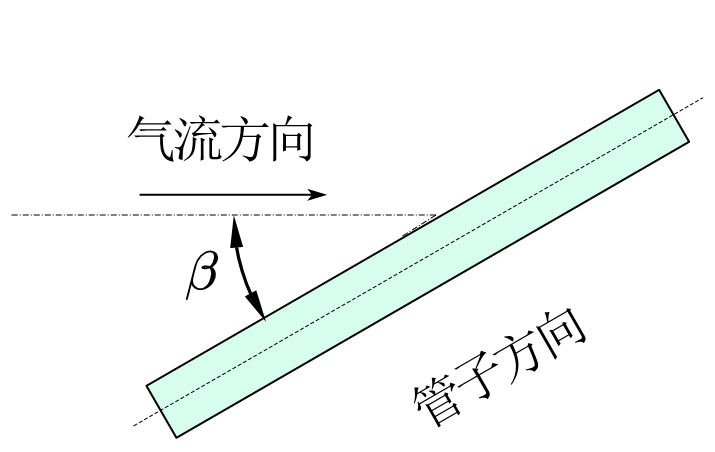
\includegraphics[width=0.4\textwidth]{img/水流角度.png}
   	\caption{流体横掠单管的示意图}\label{fig:shuiliujiaodu}
   \end{figure}
   
   \subsection{圆柱体表面温度模型}
   本模型的目标是已知圆柱体内部温度$T_o$和圆柱体外部海水温度$T_r$,求得圆柱体表面温度$T_s$。
   
   装载服务器的圆柱体可看成圆筒。设一内、外半径分别为$r_1$和$r_2$的单层圆筒壁,圆筒壁的热导率k为常数。
   
   \begin{wrapfigure}{l}{4cm}
   	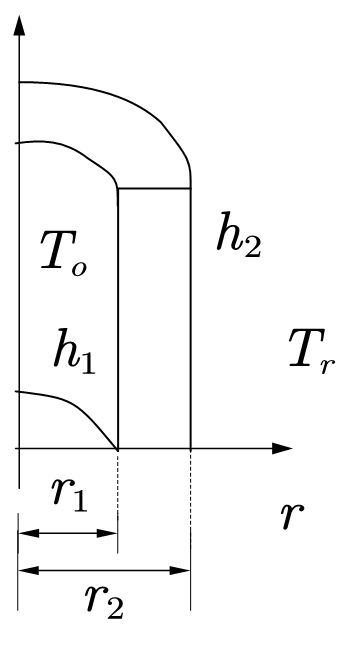
\includegraphics[width=3.5cm]{img/圆筒传热.png}
   \end{wrapfigure}
   圆筒壁内、外表面均给出第三类边界条件,即已知$r=r_1$一侧流体的温度为$T_o$,对流传热
   的表面传热系数为$h_1$ ;$r=r_2$一側流体的温度为$T_r$,表面传热系数为$h_2$,由文献\upcite{传热学}可以得到热流体通过单位管长圆简壁传给冷流体的热流量:
   \begin{equation}
   q_{l}=\frac{T_o-T_r}{\frac{1}{h_{1} \pi d_{1}}+\frac{1}{2 \pi \lambda} \ln \frac{d_{2}}{d_{1}}+\frac{1}{h_{2} \pi d_{2}}} = k_{l}\left(T_o-T_r\right)
   \label{ql}
   \end{equation}
   
  其中$$
  \frac{1}{k_{l}}=\frac{1}{h_{1} \pi d_{1}}+\frac{1}{2 \pi \lambda} \ln \frac{d_{2}}{d_{1}}+\frac{1}{h_{2} \pi d_{2}}
  $$
  $k_{l}$表示热、冷流体之间温度相差$1^{\circ} C$ 时,单位时间内通过单位长度圆
  \\
  \\
  筒壁的传热量,单位是$W/(mK)$。
  圆柱体表面温度$T_s$可由下式得到:
  \begin{equation}
  T_{s}=T_r+q_{l} \frac{1}{h_{2} \pi d_{2}}
  \label{ts}
  \end{equation}
   联立式\eqref{ql}\eqref{ts}得到:
   \begin{equation}
   T_s=T_{r}+\frac{T_{0}-T_{r}}{h_{2} d_{2}\left(\frac{1}{h_{1} d_{1}}+\frac{1}{2 \lambda} \ln \frac{d_{2}}{d_{1}}\right)+1}
   \label{Ts}
   \end{equation}
   
   使用matlab进行仿真,得到图\ref{wendufenbu}
   \begin{figure}[H]
   	\centering
   	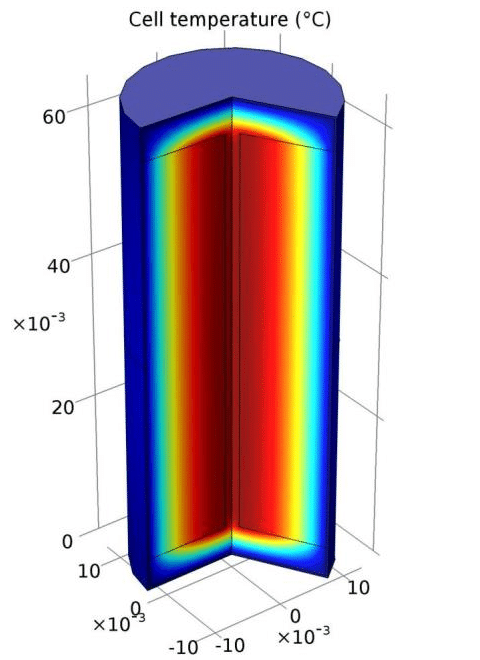
\includegraphics[width=0.4\textwidth]{img/温度分布.png}
   	\caption{圆柱体内温度分布图}
   	\label{wendufenbu}
   \end{figure}
   
   
	\section{问题一的求解}
	\subsection{负反馈稳定状态的定义}
	从公式\eqref{Ts}可以看出,圆柱体与海水的传热系数$h_2$会影响表面温度$T_s$,而由Ra数的定义公式\eqref{Ra}和Nu数的计算公式\eqref{Nu1}\eqref{Nu2}可以得知,表面温度$T_s$反过来影响传热系数$h_2$,即形成了负反馈,最终必然形成一个稳定状态;
   \begin{figure}[H]
		\centering
		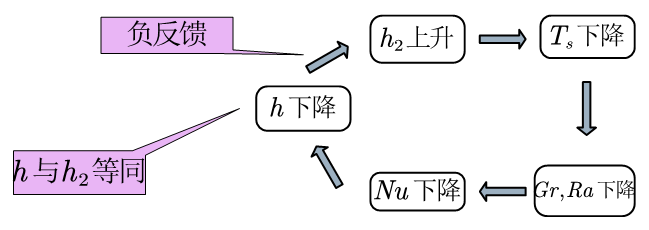
\includegraphics[width=0.7\textwidth]{img/循环图.png}
		\caption{传热循环图}
		\label{fig:xunhuantu}
	\end{figure}
	\subsection{稳定状态的求解(遍历搜索逼近法)}
	使用遍历搜索逼近法求解此稳定状态的步骤如下:
	
	\textbf{Step 1} 探究材料导热系数对稳定状态的影响,作出$T_s$随材料导热系数的变化曲线:
	\begin{figure}[H]
		\centering
		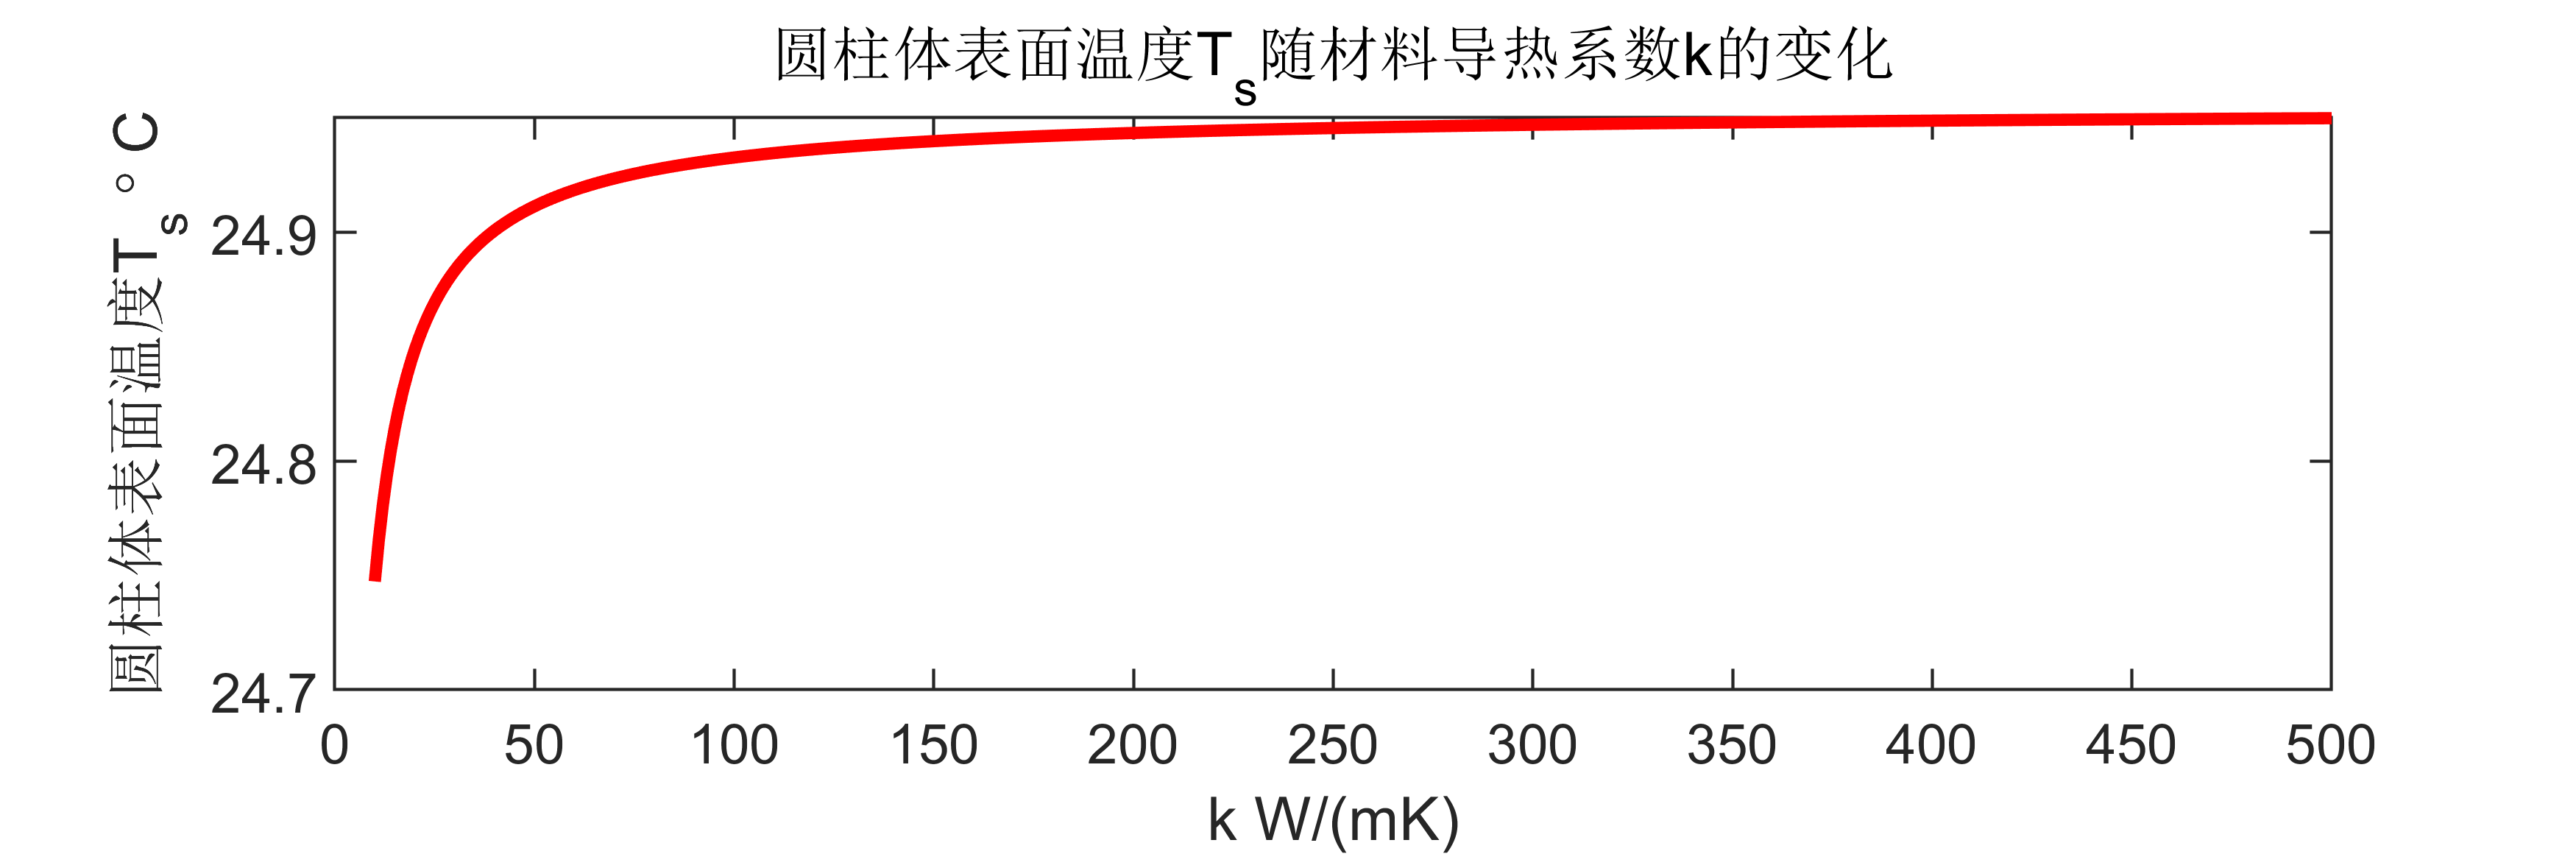
\includegraphics[width=0.8\textwidth]{img/表面温度随材料导热系数的变化.png}
		\label{fig:chailiao}
	\end{figure}
 	由图得知,材料导热系数大范围变化时,$T_s$变化很小(<$0.3^{\circ} C$),因此材料导热系数对平衡状态的影响可以忽略。
	
	\textbf{Step 2} 圆筒内空气与内壁的传热系数$h_1=10 \sim 100  W/(m^2 K)$,为获得最大服务器数量,取$h_=10  W/(m^2 K)$。假设材料为铁,圆筒外直径$d_2$为1m,圆筒外壳厚度为0.1m,内直径$d_1$为0.9m,铁的导热系数$\lambda = 80 W/(mK) $。
	
	\textbf{Step 3} 设置圆筒外海水与外表面的传热系数$h_2$的数值梯度,$h_2=100:10:10000   W/(m^2 K)$,即起始$h_2$为100,以10为间隔,终值为10000。
	
	\textbf{Step 4} 以$h_2$计算表面温度$T_s$,代入Ra数的定义公式\eqref{Ra}和Nu数的计算公式\eqref{Nu1}\eqref{Nu2},再根据公式\eqref{Nu}计算传热系数$h$.
	
	\textbf{Step 5} 当$h_2$和$h$的差值的绝对值小于某个值时,我们即可认为达到平衡状态。最后可计算出平衡状态时的服务器数量,即为最大服务器数量。
   \subsection{求解结果}
   结果如下表,其中强迫对流情况下的数据是在海水流速$u=1m/s$的情况下求得的。
   \begin{table}[htbp]
   	\centering
   	\begin{tabularx}{0.9\textwidth}{@{}c *3{>{\centering\arraybackslash}X}@{}}
   		\toprule[1.5pt]
   		对流状态  & 传热系数$h ( W/(m^2 K)) $&$表面温度Ts (^{\circ} C)$ & 最大服务器数量N \\
   		\midrule
   		自然对流  & 230   & 36    & 282 \\
   		强迫对流  & 1900  & 24    & 572 \\
   		\bottomrule[1.5pt]  
   	\end{tabularx}%
   	\label{tab:addlabel}%
   \end{table}%
   
   \section{问题二的求解}
   \subsection{容器形状的选择}
   水底的压力是可怕的,经过多重考虑最终将这套设备设计为圆柱体。是因为任何矩形都会因为海水压力的问题导致损坏,而圆形可以尽可能地降低压力。因此长方体不在考虑之列,而只考虑圆柱体。
   \subsection{结构的选择}
   考虑圆柱体上的结构,结构形态对散热的影响体现在提高了接触面积。由公式
   \begin{equation}
   N=\frac{Nu k(T_s-T_r)S}{L P}
   \end{equation}
   可知,服务器数量与表面积成正比。
   
   \subsubsection{翅片结构}
   对翅片而言,主要有3种因素\upcite{王任远2013散热器空气侧百叶窗翅片结构参数优化}影响表面积:
   
   (1) 翅片高度:增加翅片高度,将增加外表面积,但该参数受到了以下因素的限制。翅片高度影响质量流量这一基本参数,该参数影响传热和压力降;整体型翅片的制造限制要比对锯齿型翅片管的限制得多;翅片效率下降,同样,整体型翅片要比锯齿型翅片下降严重;对于翅片高度小于12 mm 的翅片,推荐使用整体型螺旋翅片。如保持其它参数不变,仅增加翅片高度,则换热器成本首先下降,然后不变,最后又开始增加,这是由于换热面积的增加量被较大的管间距效应、较低的气体流速、较低的翅片效率和较低的流体渗透率所抵消的缘故。
   
   (2) 翅片厚度:较小的翅片厚度可以带来较高的翅片密度,但是同时也降低了翅片效率,降低了结构刚度。最小翅片厚度通常为0.9 mm,如用以处理腐蚀性/润滑流体或高温流体时,需使用厚度更大的翅片,厚度可达4.2 mm,而对于小直径情形,将受到一些限制。最常用的翅片厚度为1.2 mm。
   
   (3) 翅片密度(间隔):为了获得单位管长的最大外表面积,需使用最高的允许翅片密度,但是过高翅片密度带来压降过大,气体不完全渗透,污垢加重等问题。
   
	\subsubsection{格栅结构}
   另外可以利用内外双散热格栅的方式进行海水交换以解决设备的散热问题,但是外部的格栅很容易因为海洋生物的堆积而出现故障。所以可以只保留内部格栅并采用海水吸入的方式来保证散热的效果。虽然这个方案可以有效的降低成本并且保证散热的高效性,但是海洋生物也会因此进入内部格栅而堆积。
   
   为了解决这个问题,可以在格栅内部的管道覆盖光滑的涂层并且放置电解产氯的设备,其产生的氯气足以杀死海水中的细菌等。
   
   
   \section{问题三的求解}
   \subsection{最佳材料的评价}
   \subsubsection{数据预处理}
   同时增大的压力会对集装箱外壳的耐压能力提出更高的要求;值得注意的是海水本身是一种强的腐蚀介质,直接与海水接触的各种金属结构物都不可避免地受到海水的腐蚀。我们的目标是在问题2的基础上进一步选择合适的材料和海底深度进行优化设计,进一步提高散热效果,并尽可能降低成本,提高使用年限。
   
   较深的海水具有较低的温度,能取得更好的散热效果,但由图\ref{wendushendu}可知,在海洋表层(深度<300m),温度变化并不大(20 - 24),因此此处不考虑因深度变化引起的温度变化的影响。
   	\begin{figure}[H]
   	\centering
   	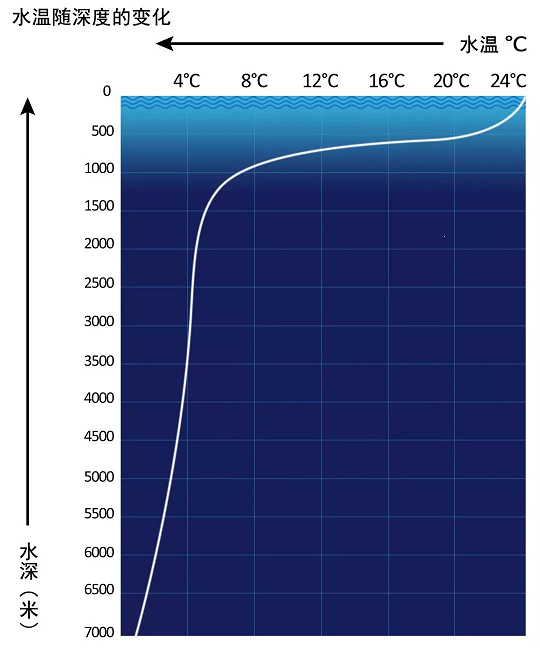
\includegraphics[width=0.4\textwidth]{img/温度深度.png}
   	\caption{海水温度随深度的变化}
   	\label{wendushendu}
   	\end{figure}
   分析附件中的数据,附件中所给的数据主要有,材料,材料组成,密度,弹性模量,屈服强度,拉抗强度,海水电位,遭受的腐蚀类型,应用和特别提醒。
   
   首先排除一些密度不够大,强度低,不耐腐蚀的材料,如木材等,最后只保留金属材料,在金属材料里,贵金属如金银和纯金属铅等不在考虑之列,复合材料在目前备受关注,并且它也具有极强的抗腐蚀性以及相对优异的成本优势,但是它并不能承受过大的水压,因此无法被使用。最后保留6种类型的金属材料,即铝合金、铜和铜合金、镍合金、铁类、钛和钛合金、不锈钢。
   
   通过取平均值汇总每一大类的密度,弹性模量,屈服强度,拉抗强度,海水电位,对于范围值,取其中值。对于钛合金,海水电位相比之下太小,导致最后结果不准确,因此钛合金的海水电位取其极值。
   
   由于还需要考虑成本,因此还要加入每种金属的价格。
   
   求得的数据表如下:
	\begin{table}[H]
	\centering
	\caption{各金属类的相关数据}
	\begin{tabularx}{0.9\textwidth}{@{}c *7{>{\centering\arraybackslash}X}@{}}
		\toprule[1.5pt]
		& 价格 $USD/t$    & 密度$kg/m^3$    & 单位体积价格 $USD/m^3$ & 弹性模量$10^6  E (psi)$ & 屈服强度 $O_y (ksi)$  & 拉伸强度 $O_u (ksi)$  & 海水电位$ ref. Ag-AgCl (V)$ \\
		\midrule
		铝合金   & 2328  & 2740  & 6379  & 10    & 51    & 57    & .0.85 \\
		铜和铜合金 & 9187  & 8447  & 77606 & 17    & 65    & 87    & 0.23 \\
		镍合金   & 17692 & 8470  & 149852 & 28    & 125   & 143   & 0.07 \\
		铁类   & 700   & 7766  & 5436  & 29    & 122   & 144   & 0.63 \\
		钛和钛合金 & 11214 & 4470  & 50130 & 16    & 122   & 132   & 0.06 \\
		不锈钢   & 2142  & 7935  & 16997 & 28    & 97    & 136   & 0.29 \\
		\bottomrule[1.5pt]  
	\end{tabularx}
	\end{table}%
  
  
  将上表数据进行归一,统一归一到[0,1]区间,得到:
	\begin{table}[H]
		\centering
		\caption{归一化数据}
		\begin{tabularx}{0.9\textwidth}{@{}c *5{>{\centering\arraybackslash}X}@{}}
			\toprule[1.5pt]
			& 单位体积价格    & 弹性模量 & 屈服强度  & 拉伸强度  & 海水电位 \\
			\midrule
			铝合金   & 0.020819 & 0.078125 & 0.087628866 & 0.081545064 & 0.399061 \\
			铜和铜合金 & 0.253283 & 0.1328125 & 0.111683849 & 0.124463519 & 0.107981 \\
			镍合金   & 0.489073 & 0.21875 & 0.214776632 & 0.204577969 & 0.032864 \\
			铁类    & 0.017742 & 0.2265625 & 0.209621993 & 0.206008584 & 0.295775 \\
			钛和钛合金 & 0.16361 & 0.125 & 0.209621993 & 0.188841202 & 0.028169 \\
			不锈钢   & 0.055473 & 0.21875 & 0.166666667 & 0.194563662 & 0.13615 \\
			\bottomrule[1.5pt]  
		\end{tabularx}%
		\label{}%
	\end{table}%
  其中单位体积价格表征成本,弹性模量,屈服强度,拉伸强度表征抗压能力,我们假设这3个量对抗压能力的影响相同,即将3个数求平均值。海水电位表征抗腐蚀能力,电位的绝对值越低说明抗腐蚀能力越强。对价格和海水电位求倒数再归一到[0,1]区间,分别表示成本量和抗腐蚀能力。
  得到标准化的数据:
  \begin{table}[htbp]
  	\centering
  	\caption{表征成本,抗压能力,抗腐蚀能力的标准化数据}
  	\begin{tabularx}{0.9\textwidth}{@{}c *3{>{\centering\arraybackslash}X}@{}}
  		\toprule[1.5pt]
  		& 成本    & 抗压能力  & 抗腐蚀能力 \\
  		\midrule
  		铝合金   & 0.357 & 0.082 & 0.028 \\
  		铜和铜合金 & 0.029 & 0.123 & 0.105 \\
  		镍合金   & 0.015 & 0.213 & 0.344 \\
  		铁类   & 0.419 & 0.214 & 0.038 \\
  		钛和钛合金 & 0.045 & 0.174 & 0.401 \\
  		不锈钢   & 0.134 & 0.193 & 0.083 \\
  		\bottomrule[1.5pt]  
  	\end{tabularx}%
  	\label{biaozhunhuashujv}%
  \end{table}%
  
  \subsubsection{层次分析法求解最佳材料}
  构造判断矩阵A:通常情况下,成本,抗压能力,抗腐蚀能力是同等重要的因素,因此抗压构造判断矩阵A:
  $$
  A=\left[ \begin{matrix}
  1&		1&		1\\
  1&		1&		1\\
  1&		1&		1\\
  \end{matrix} \right] 
  $$
  计算一致性指标Cl
  \begin{equation}
  C I=\frac{\lambda_{\max }-n}{n-1}
  \end{equation}
  计算一致性比例CR\upcite{数学模型}
  \begin{equation}
  R I=\frac{\lambda_{\max }^{\prime}-n}{n-1}
  \end{equation}

  \begin{equation}
  C R=\frac{C I}{R I}
  \end{equation}
  当CR<0.10时,认为判断矩阵的一致性是可以接受的,否则应对判断矩阵作适当修正。
  
  由判断矩阵A计算CR = -4.2701e-16,判断矩阵的一致性是可以接受的。
  
  设B层中与A,相关的因素的成对比较判断矩阵在单排序中经一致性检验,求得
  单排序一致性指标为$C I(j),(j=1, \cdots, m)$,相应的平均随机一致性指标为RI(j)/(
  (CI(j)、RI(j)已在层次单排序时求得),则B层总排序随机一致性比例为
  \begin{equation}
  C R=\frac{\sum_{j=1}^{m} C I(j) a_{j}}{\sum_{j=1}^{m} R I(j) a_{j}}
  \end{equation}
  
  模型框图如下:
  	\begin{figure}[H]
  	\centering
  	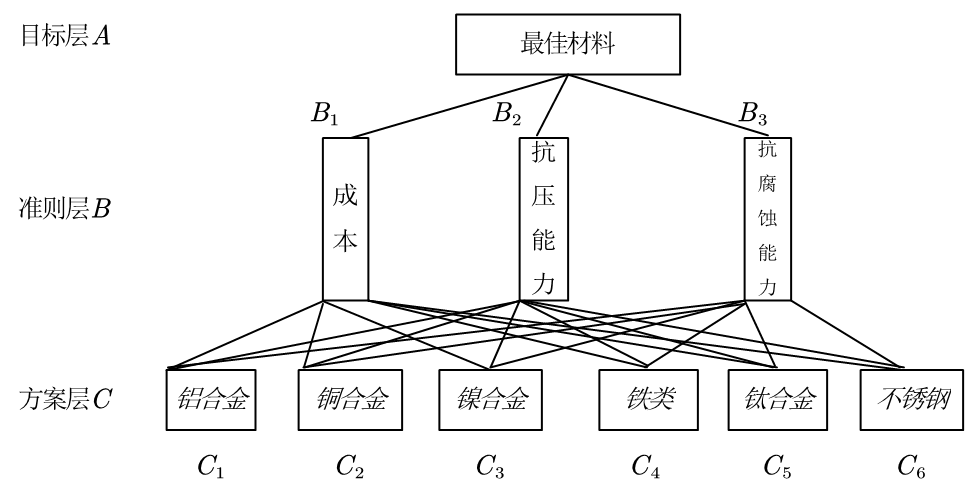
\includegraphics[width=0.8\textwidth]{img/层次分析法图.png}
  	\label{fig:ccfxft}
  \end{figure}
  根据表\ref{biaozhunhuashujv}计算方案层的判断矩阵:
  \begin{table}[H]
  	\centering
  	\caption{方案层的判断矩阵}
  	\begin{tabular}{ccccccc}
  		\toprule[1.5pt]
  		$B1$    & $C_1$     & $C_2$     & $C_3$      & $C_4$      & $C_5$      & $C_6$  \\
  		$C_1$     & 1.00  & 12.17 & 23.49 & 0.85  & 7.86  & 2.66 \\
  		$C_2$     & 0.08  & 1.00  & 1.93  & 0.07  & 0.65  & 0.22 \\
  		$C_3$     & 0.04  & 0.52  & 1.00  & 0.04  & 0.33  & 0.11 \\
  		$C_4$     & 1.17  & 14.28 & 27.57 & 1.00  & 9.22  & 3.13 \\
  		$C_5$     & 0.13  & 1.55  & 2.99  & 0.11  & 1.00  & 0.34 \\
  		$C_6$     & 0.38  & 4.57  & 8.82  & 0.32  & 2.95  & 1.00 \\
  		\toprule[1.5pt]
  		$B_2$    & $C_1$     & $C_2$     & $C_3$      & $C_4$      & $C_5$      & $C_6$  \\
  		$C_1$     & 1.00  & 0.67  & 0.39  & 0.39  & 0.47  & 0.43 \\
  		$C_2$     & 1.49  & 1.00  & 0.58  & 0.57  & 0.70  & 0.64 \\
  		$C_3$     & 2.58  & 1.73  & 1.00  & 0.99  & 1.22  & 1.10 \\
  		$C_4$     & 2.60  & 1.74  & 1.01  & 1.00  & 1.23  & 1.11 \\
  		$C_5$     & 2.12  & 1.42  & 0.82  & 0.82  & 1.00  & 0.90 \\
  		$C_6$     & 2.35  & 1.57  & 0.91  & 0.90  & 1.11  & 1.00 \\
  		\toprule[1.5pt]
  		$B_3$    & $C_1$     & $C_2$     & $C_3$      & $C_4$      & $C_5$      & $C_6$  \\
  		$C_1$     & 1.00  & 0.27  & 0.08  & 0.74  & 0.07  & 0.34 \\
  		$C_2$     & 3.70  & 1.00  & 0.30  & 2.74  & 0.26  & 1.26 \\
  		$C_3$     & 12.14 & 3.29  & 1.00  & 9.00  & 0.86  & 4.14 \\
  		$C_4$     & 1.35  & 0.37  & 0.11  & 1.00  & 0.10  & 0.46 \\
  		$C_5$     & 14.17 & 3.83  & 1.17  & 10.50 & 1.00  & 4.83 \\
  		$C_6$     & 2.93  & 0.79  & 0.24  & 2.17  & 0.21  & 1.00 \\
  		\bottomrule[1.5pt]
  	\end{tabular}%
  	\label{}%
  \end{table}%
  层次总排序的结果如下:
 \begin{table}[H]
 	\centering
 	\caption{层次总排序}
 	\begin{tabular}{c|c|ccc|c}
 		\toprule[1.5pt]
 		\multicolumn{2}{c|}{准则} & 成本    & 抗压能力  & 抗腐蚀能力 & \multirow{2}[4]{*}{总权值排序} \\
 		\cmidrule{1-5}    \multicolumn{2}{c|}{准则层权值} & 0.33  & 0.33  & 0.33  &  \\
 		\midrule[1.5pt]
 		\multirow{6}[2]{*}{方案层单排序权值} & 铝合金   & 0.36  & 0.08  & 0.03  & 0.16 \\
 		& 铜和铜合金 & 0.03  & 0.12  & 0.10  & 0.09 \\
 		& 镍合金   & 0.02  & 0.21  & 0.34  & 0.19 \\
 		& 铁类    & 0.42  & 0.21  & 0.04  & 0.22 \\
 		& 钛和钛合金 & 0.05  & 0.17  & 0.40  & 0.21 \\
 		& 不锈钢   & 0.13  & 0.19  & 0.08  & 0.14 \\
 		\bottomrule[1.5pt]
 	\end{tabular}%
 	\label{}%
 \end{table}%
  根据层次总排序权值,可知最佳材料应该是铁类。最后再根据铁类中的具体某一类,根据制造成本等因素具体选择。
  
  另外,我们可以看到,铁类和钛合金的得分相近,考虑到钛合金优秀的抗腐蚀能力,因此可以以钢铁为主要材料,外壳以钛合金为涂料,这样即节约成本,又提高抗腐蚀能力,同时保证抗压能力。为了防止由于涂层脱落导致腐蚀的发生,还可以采用了阴极保护的手法。
 
%   \subsection{最佳深度的评价}
%    容器的设计方面,其可以实现 150m 深度安全运行,并且极限深度为 290m,但是测试过程中部署的深度仅为 100m。相较于第一阶段部署深度 20m 且高达 75mm 的涂层而言,第二阶段已经大幅度提高其性能,实现 100m 部署深度并且涂层厚度仅为 19mm。
    
   \section{问题四的求解}
   
    潮汐和季节会改变局部水位和温度,并带来暂时性的海水流动,可能对数据中心的散热带来一定影响。温度变化主要是由于季节改交造成的,此因素需要结合问题1进行
    分析,在问题1的模型上加入温度变化这个因子;海水流动的原因与潮汐和季节改变都有关,海水流动会造成流速加快,会让海水降温更快,即考虑强制对流情况下海水流速对散热的影响。另外,潮汐可能改变海水来流角度,对结果也有一定的影响。
    \subsection{海水温度变化对结果的影响}
    考虑海水温度对结果的影响时,应该采用自然对流模型,将海水温度的变化加入问题1中的遍历搜索逼近算法,即设置2层循环遍历,求得各个温度下的服务器最大数量;
    结果如图\ref{fwqslswd}
    \begin{figure}[H]
    	\centering
    	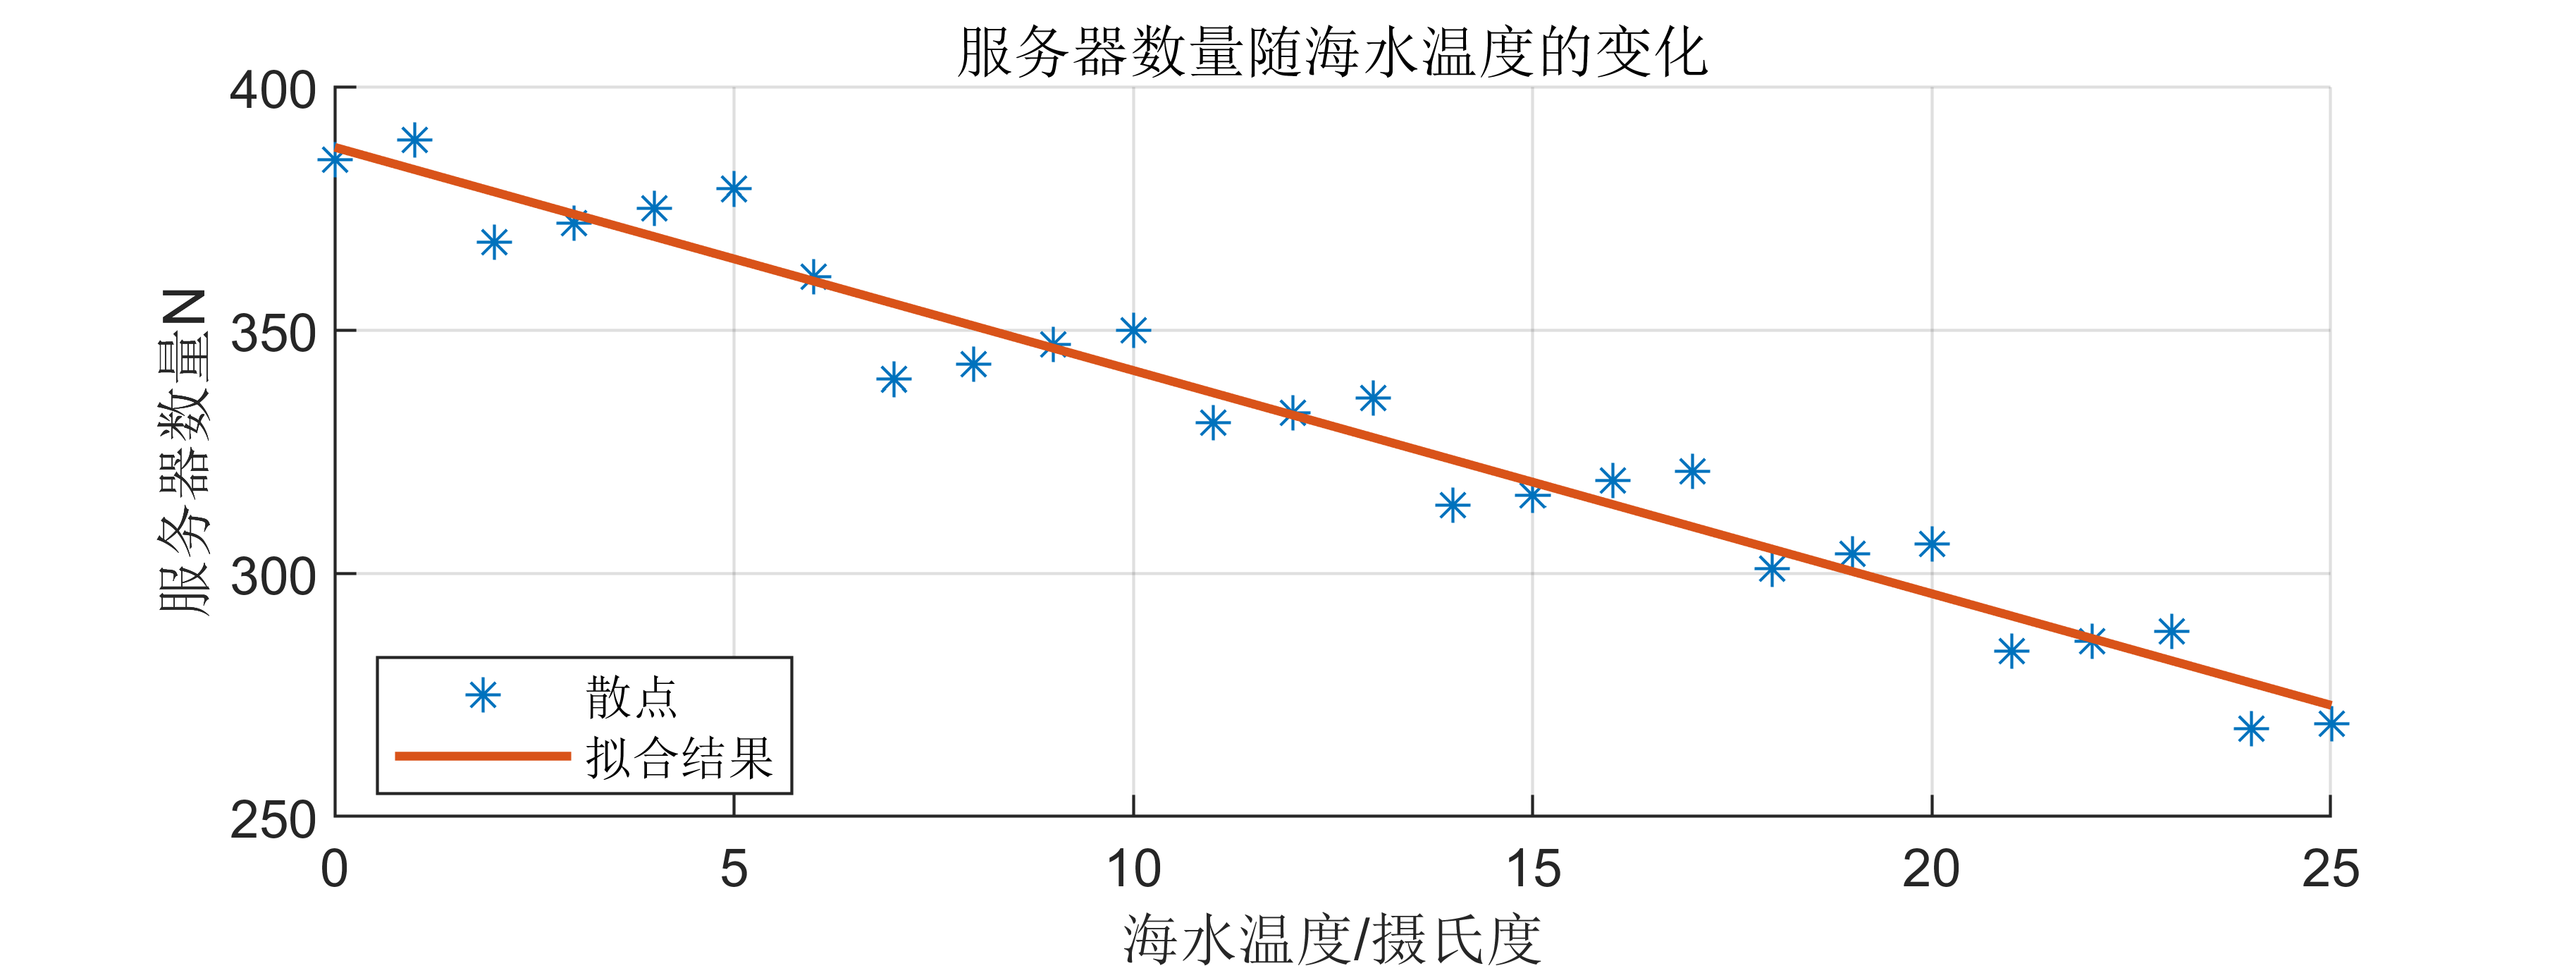
\includegraphics[width=0.8\textwidth]{img/服务器数量随温度变化曲线及拟合结果.png}
    	\label{fwqslswd}
    \end{figure}
    由图可以看出,随着海水温度的升高(从0到25摄氏度),服务器最大数量从385下降到265台。两者之间呈现负的一次函数关系。
    
    
    \subsection{海水流速变化对结果的影响}
    考虑海水温度对结果的影响时,由于海水的流动,应该采用强制对流模型,将海水流速的变化加入问题1中的遍历搜索逼近算法,同样即设置2层循环遍历,求得各个流速值下的服务器最大数量;
    结果如图\ref{fwqsls}
    \begin{figure}[H]
    	\centering
    	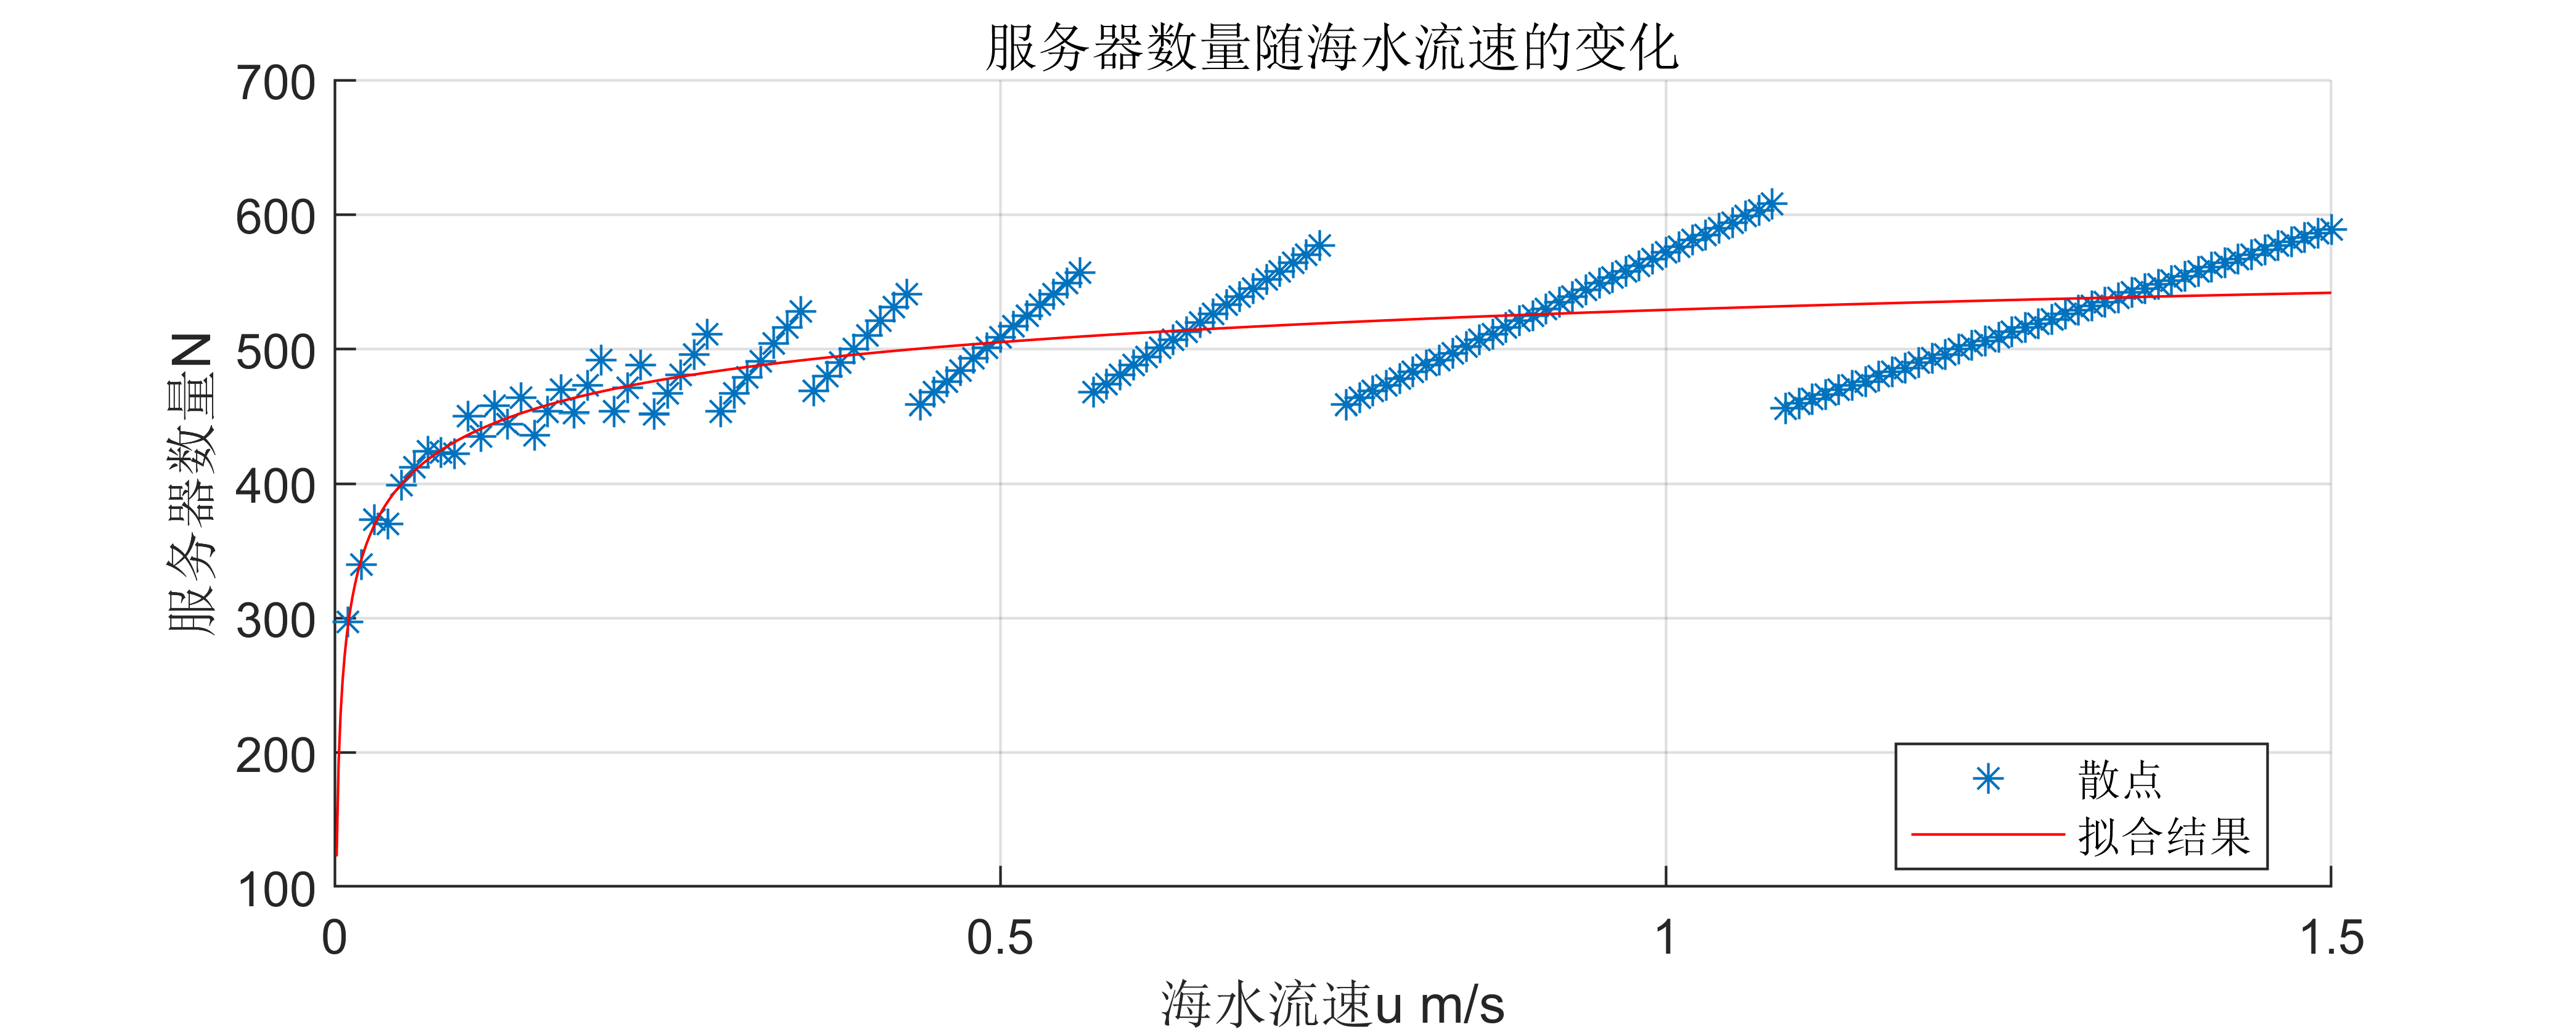
\includegraphics[width=0.8\textwidth]{img/服务器数量随流速变化曲线及拟合结果2.png}
    	\label{fwqsls}
    \end{figure}
   对图中的散点,呈现分段的现象,这种现象是由于计算强制对流状态时,使用的是公式\eqref{Nu2},公式本身是分段的。因此对散点进行拟合,观察曲线趋势可以得到服务器数量与流速呈现对数关系,在流速较小段,最大服务器数量随流速的增大而迅速上升,在流速大于$0.5m/s$之后,服务器最大数量上升缓慢,保持在500-600台之间。
   
   呈现对数关系的原因分析:
   
   在强制对流传热过程中,由于流体各部分温度的差异,将发生自然对流。这里的计算没有考虑自然对流的影响,视为纯强制对流传热。若在强制对流中自然对流因素不
   可忽略,这种流动称为自然与强制并存的混合流动。
   
   一般情况下可以认为$Gr/Re^2 \geq 0.1$时,就不能忽略自然对流的影响;如果$Gr/Re^2\geq 10$
   则可作为纯自然对流看待,而忽略受迫对流.
   
   当流速很小时,主要还是自然对流占优,当稍微增大,强制对流占优,在此阶段散热能力迅速提高;在流速很大时,散热能力已经接近最大,因此服务器数量上升缓慢。
   
   \subsection{海水来流角度对结果的影响}
   来流角度对服务器数量的影响也较大。当海水横掠单管时,主要存在紊流,促进了传热,传热系数$h$升高,服务器数量也增大;当海水流向平行于圆柱体轴时,主要是层流,传热系数没有紊流的大。
   由公式\eqref{jd}服务器最大数量随海水来流角度的变化曲线如图\ref{fwqslsjd},由图可知,当海水流向平行于圆柱体轴时,最大服务器数量为$250+$。
   \begin{figure}[H]
   	\centering
   	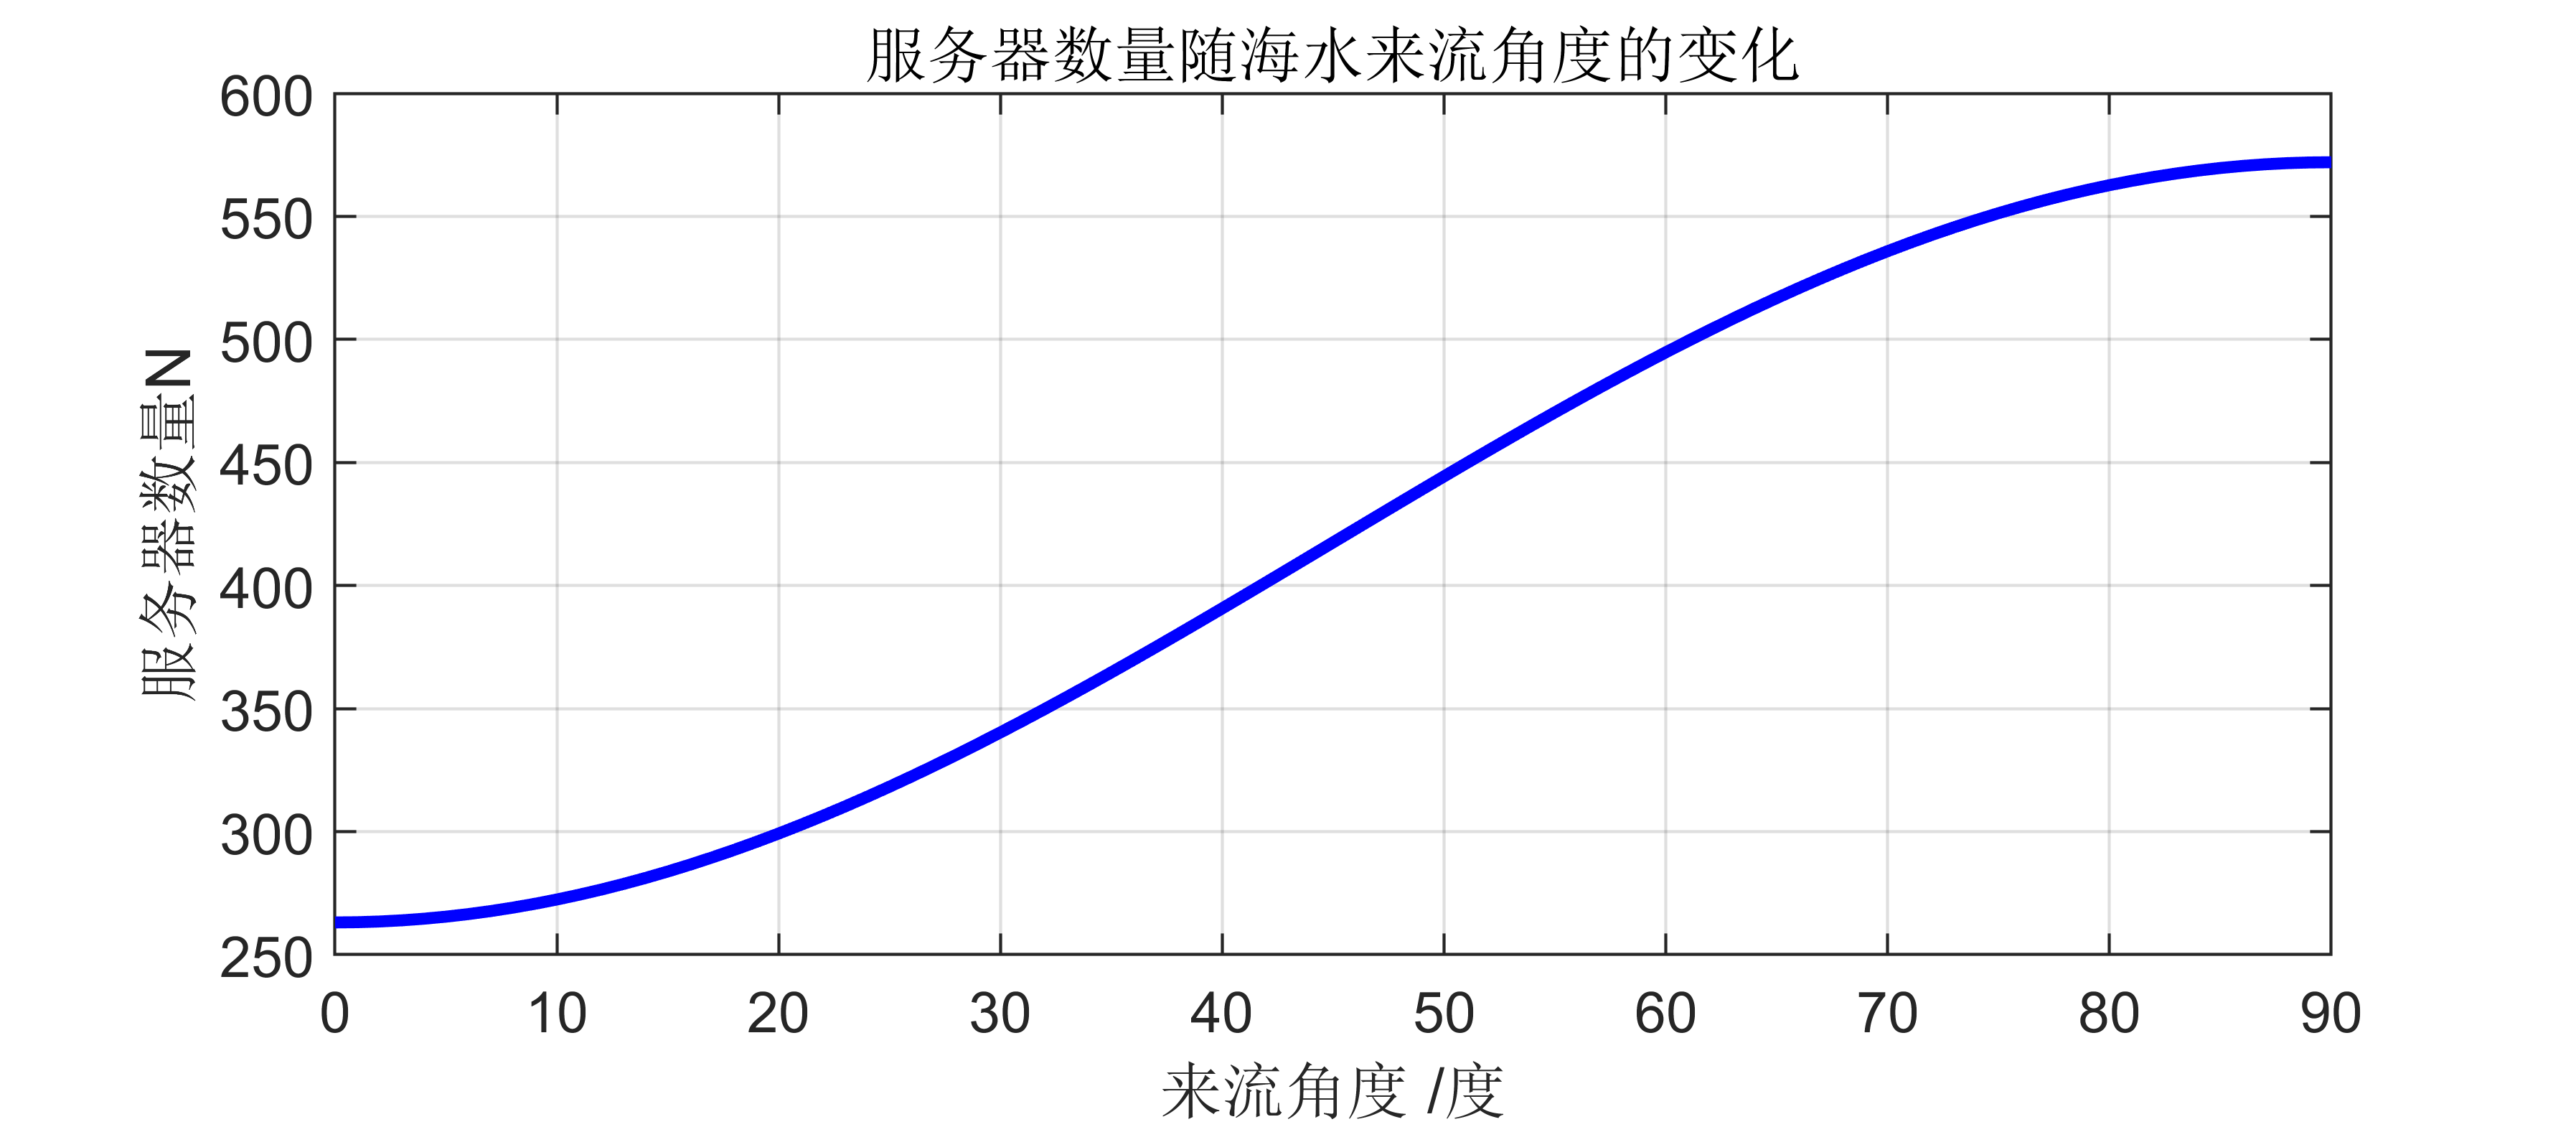
\includegraphics[width=0.8\textwidth]{img/服务器数量随海水来流角度的变化.png}
   	\caption{服务器数量随海水来流角度的变化}
   	\label{fwqslsjd}
   \end{figure}  

 \section{模型的评价}
 \subsection{模型的优点}
	 \begin{itemize}
	 	\item 综合考虑了圆柱体内部热传导和圆柱体外部热对流,同时建立热传导和热对流之间的联系,即热传导影响圆柱体表面温度,表面温度的变化又通过热对流反过来影响热传导;
	 	\item 建立了传热的稳定状态模型,通过遍历搜索逼近算法求得稳定状态量;
	 	\item 评价了各个因素如海水温度、海水流速、来流角度、外壳材料导热系数对最大服务器数量的影响;
	 \end{itemize}
 \subsection{模型的缺点}
 	\begin{itemize}
	 	\item 对圆柱体内部热传导只进行了简单分析,将内部温度看成统一的$80^\circ C$,实际上,圆柱体内部温度是渐变的;并且如果服务器不是放在中心,而是紧贴外壳分布,模型需要另作讨论。
	 	\item 圆柱体内部空气与外壳之间的传热系数$h_1$会随着温度的改变而改变,对结果有一定的影响,本文未考虑此因素。
	 	\item 未对数据中心放置的最佳深度作详细的讨论。

   \end{itemize}

 \newpage

 \section{建议信}
    \noindent 尊敬的微软公司:
    
    知悉贵公司在部署海下数据中心,对于海底数据中心,如何在有限的体积内存放更多的服务器且保证服务器工作过程中向海水中正常快速的散热是一项非常有挑战性的问题。我们团队对海底数据中心进行了优化设计,希望给贵公司的海底数据中心的外壳散热提供设计方案提供以下建议:
    
    (1) 容器结构设计:外形采用圆柱形,抗压效果最好;
    
    利用内外双散热格栅的方式进行海水交换以解决设备的散热问题,但是外部的格栅很容易因为海洋生物的堆积而出现故障,可以只保留内部格栅并采用海水吸入的方式来保证散热的效果。并在格栅内部的管道覆盖光滑的涂层并且放置电解产氯的设备。
    
    (2) 容器材料选择:根据我们层次分析法得出的分数,采用钢铁为主要材料,加以钛合金为涂层,能够节约成本同时保证抗压和抗腐蚀能力;
    
    (3) 服务器承载力:对于直径1m,长12m的圆柱体,自然对流情况下最大服务器数量为282台,建议部署服务器是不要超过该值(按体积比例计算对应的值)。
    
    (4) 容器放置深度:在 150m 深度可以安全运行,并且极限深度为 290m,但是部署的最佳深度建议为 100m 。
    
    此致
    
    \noindent 敬礼
    
   \null\hfill 数模团队 
   
   \null\hfill 2020.4.18
    
    \newpage
    
 \section{参考文献}
	%\addcontentsline{toc}{section}{参考文献}
	\bibliographystyle{unsrt}
	\bibliography{bib/ref.bib}
    
    
    
    
    
    
    
    
    
    
    
    
    
    
    \section{附录}
 	\appendix
 	\section{Matlab程序}
 	\textbf{水的物性参数}
 	\begin{lstlisting}[language=matlab]
 	%温度t/c	密度      比热容	     热导率	 运动黏度   动力黏度	普朗特数
 	% t/c   p kg/m3  Cp kJ/(kg K)   k W/(m K)   V m/s    v Pa s   Pr
 	waterchanshu = [0	999.9	4.212	0.551	1.789E-06	0.001788	13.67
 	1	999.9	4.210	0.553	1.741E-06	0.0017398	13.26
 	2	999.9	4.208	0.556	1.692E-06	0.0016916	12.84
 	3	999.9	4.206	0.558	1.644E-06	0.0016434	12.43
 	4	999.8	4.204	0.560	1.596E-06	0.0015952	12.01
 	5	999.8	4.202	0.563	1.548E-06	0.001547	11.60
 	6	999.8	4.199	0.565	1.499E-06	0.0014988	11.18
 	7	999.8	4.197	0.567	1.451E-06	0.0014506	10.77
 	8	999.7	4.195	0.569	1.403E-06	0.0014024	10.35
 	9	999.7	4.193	0.572	1.354E-06	0.0013542	9.94
 	10	999.7	4.191	0.574	1.306E-06	0.001306	9.52
 	11	999.6	4.190	0.577	1.276E-06	0.0012758	9.27
 	12	999.4	4.189	0.579	1.246E-06	0.0012456	9.02
 	13	999.3	4.189	0.582	1.216E-06	0.0012154	8.77
 	14	999.1	4.188	0.584	1.186E-06	0.0011852	8.52
 	15	999.0	4.187	0.587	1.156E-06	0.001155	8.27
 	16	998.8	4.186	0.589	1.126E-06	0.0011248	8.02
 	17	998.7	4.185	0.592	1.096E-06	0.0010946	7.77
 	18	998.5	4.185	0.594	1.066E-06	0.0010644	7.52
 	19	998.4	4.184	0.597	1.036E-06	0.0010342	7.27
 	20	998.2	4.183	0.599	1.006E-06	0.001004	7.02
 	21	998.0	4.182	0.601	9.859E-07	0.00098375	6.86
 	22	997.7	4.181	0.603	9.658E-07	0.0009635	6.70
 	23	997.5	4.180	0.605	9.457E-07	0.00094325	6.54
 	24	997.2	4.179	0.607	9.256E-07	0.000923	6.38
 	25	997.0	4.179	0.609	9.055E-07	0.00090275	6.22
 	26	996.7	4.178	0.610	8.854E-07	0.0008825	6.06
 	27	996.5	4.177	0.612	8.653E-07	0.00086225	5.90
 	28	996.2	4.176	0.614	8.452E-07	0.000842	5.74
 	29	996.0	4.175	0.616	8.251E-07	0.00082175	5.58
 	30	995.7	4.174	0.618	8.050E-07	0.0008015	5.42
 	31	995.4	4.174	0.620	7.904E-07	0.00078668	5.31
 	32	995.0	4.174	0.621	7.758E-07	0.00077186	5.20
 	33	994.7	4.174	0.623	7.612E-07	0.00075704	5.09
 	34	994.3	4.174	0.625	7.466E-07	0.00074222	4.98
 	35	994.0	4.174	0.627	7.320E-07	0.0007274	4.87
 	36	993.6	4.174	0.628	7.174E-07	0.00071258	4.75
 	37	993.3	4.174	0.630	7.028E-07	0.00069776	4.64
 	38	992.9	4.174	0.632	6.882E-07	0.00068294	4.53
 	39	992.6	4.174	0.633	6.736E-07	0.00066812	4.42
 	40	992.2	4.174	0.635	6.590E-07	0.0006533	4.31
 	41	991.8	4.174	0.636	6.487E-07	0.00064291	4.23
 	42	991.4	4.174	0.638	6.384E-07	0.00063252	4.16
 	43	991.0	4.174	0.639	6.281E-07	0.00062213	4.08
 	44	990.6	4.174	0.640	6.178E-07	0.00061174	4.00
 	45	990.2	4.174	0.642	6.075E-07	0.00060135	3.93
 	46	989.7	4.174	0.643	5.972E-07	0.00059096	3.85
 	47	989.3	4.174	0.644	5.869E-07	0.00058057	3.77
 	48	988.9	4.174	0.645	5.766E-07	0.00057018	3.69
 	49	988.5	4.174	0.647	5.663E-07	0.00055979	3.62
 	50	988.1	4.174	0.648	5.560E-07	0.0005494	3.54
 	51	987.6	4.175	0.649	5.482E-07	0.00054145	3.49
 	52	987.1	4.175	0.650	5.404E-07	0.0005335	3.43
 	53	986.6	4.176	0.651	5.326E-07	0.00052555	3.38
 	54	986.1	4.176	0.652	5.248E-07	0.0005176	3.32
 	55	985.6	4.177	0.654	5.170E-07	0.00050965	3.27
 	56	985.1	4.177	0.655	5.092E-07	0.0005017	3.21
 	57	984.6	4.178	0.656	5.014E-07	0.00049375	3.16
 	58	984.1	4.178	0.657	4.936E-07	0.0004858	3.10
 	59	983.6	4.179	0.658	4.858E-07	0.00047785	3.05
 	60	983.1	4.179	0.659	4.780E-07	0.0004699	2.99
 	61	982.6	4.180	0.660	4.717E-07	0.00046352	2.95
 	62	982.0	4.181	0.661	4.654E-07	0.00045714	2.90
 	63	981.5	4.181	0.662	4.591E-07	0.00045076	2.86
 	64	981.0	4.182	0.663	4.528E-07	0.00044438	2.81
 	65	980.5	4.183	0.664	4.465E-07	0.000438	2.77
 	66	979.9	4.184	0.664	4.402E-07	0.00043162	2.73
 	67	979.4	4.185	0.665	4.339E-07	0.00042524	2.68
 	68	978.9	4.185	0.666	4.276E-07	0.00041886	2.64
 	69	978.3	4.186	0.667	4.213E-07	0.00041248	2.59
 	70	977.8	4.187	0.668	4.150E-07	0.0004061	2.55
 	71	977.2	4.188	0.669	4.100E-07	0.000401	2.52
 	72	976.6	4.189	0.669	4.050E-07	0.0003959	2.48
 	73	976.0	4.189	0.670	4.000E-07	0.0003908	2.45
 	74	975.4	4.190	0.670	3.950E-07	0.0003857	2.41
 	75	974.8	4.191	0.671	3.900E-07	0.0003806	2.38
 	76	974.2	4.192	0.672	3.850E-07	0.0003755	2.35
 	77	973.6	4.193	0.672	3.800E-07	0.0003704	2.31
 	78	973.0	4.193	0.673	3.750E-07	0.0003653	2.28
 	79	972.4	4.194	0.673	3.700E-07	0.0003602	2.24
 	80	971.8	4.195	0.674	3.650E-07	0.0003551	2.21
 	];
 	save waterchanshu
 	\end{lstlisting}
 	\textbf{论文的公式函数的定义}
 	\begin{lstlisting}[language=matlab]
 	function re = Re(u,L,v)
	 	re = u*L/v;
 	end
 	
 	function gr = Gr(Ts,Tr,L,v)
	 	global waterchanshu
	 	g = 9.8;
	 	%beta = 2/(Ts+Tr+273.15*2);
	 	%beta = waterchanshu((Ts+Tr)/2+1,8);
	 	beta = 0.21*10^(-3);
	 	gr = g*beta*(Ts-Tr)*L^3/(v^2);
 	end
 	
 	function ra = Ra(gr,pr)
 		ra = gr*pr;
 	end
 	
 	function nu = Nu_zhiran(ra,pr)
 		nu = (0.6+0.387*ra^(1/6)/((1+(0.559/pr)^(9/16)))^(8/27))^2;
 	end
 	
 	function nu = Nu_zhiran_jianhua(ra)
 		nu = 0.53*ra^0.25;
 	end
 	
 	function nu = Nu_qiangzhi(re,prr,prs)
	 	if re>5 && re<10^3
		 	C=0.5;
		 	n=0.5;
	 	elseif re>10^3 && re<2*10^5
		 	C=0.26;
		 	n=0.6;
		 	else 
	 	C=0.023;
		 	n=0.8;
		 	end
	 	nu = C*re^n*prr^0.37*(prr/prs)^0.25;
 	end
 	
 	function pr = Pr(Tr)
	 	global waterchanshu
	 	pr = waterchanshu(Tr+1,7);
 	end
 	
 	
 	function n = N(nu,k,Ts,Tr,S,P,L)
 		n = round(nu*k*(Ts-Tr)*S/P/L);
 	end
 	
 	function ts = findTs(to,tr,h1,h2,d1,d2,k2)
	 	ts = tr+(to-tr)./(h2*d2*(1./h1./d1+0.5./k2*log(d2./d1))+1);
	 	ts = round(ts);
 	end
 	\end{lstlisting}
 	\textbf{遍历搜索逼近算法}
 	\begin{lstlisting}[language=matlab]
 	clear 
 	clc
 	%load waterchanshu
 	global waterchanshu
 	To = 80;%圆柱体中心温度
 	Tr = 20;%海水温度
 	L = 1;%特征长度
 	u = 1;%流速
 	S = 12*pi;%表面积
 	P = 500;%功率
 	H2 = 100:10:10000;
 	h1=150;d1=0.9;d2=1;k2=80;
 	grall=[];
 	hall=[];
 	nall=[];
 	for h2 = H2
	 	ts = findTs(To,Tr,h1,h2,d1,d2,k2);
	 	Tm = round((ts+Tr)/2);%定性温度
	 	v = waterchanshu(Tm+1,5);
	 	pr = Pr(Tm);
	 	prr = Pr(Tr);
	 	prs = Pr(ts);
	 	re = Re(u,L,v);
	 	gr = Gr(ts,Tr,L,v);
	 	ra = Ra(gr,pr);
	 	%     nu = Nu_zhiran(ra,pr);
	 	%     nu = Nu_zhiran_jianhua(ra);
	 	nu = Nu_qiangzhi(re,prr,prs);
	 	k = waterchanshu(Tm+1,4);%导热系数
	 	h = k*nu/L; %传热系数
	 	
	 	if abs(h2-h)<8
		 	chazhi = abs(h2-h)
		 	n = N(nu,k,ts,Tr,S,P,L)
		 	bili = gr/(re^2)
	 	end
 	end
 	
 	\end{lstlisting}
 	\textbf{层次分析法}
 	%\lstinputlisting[language=matlab]{code/AHP.m}
 	\begin{lstlisting}[language=matlab]
 	clc,clear 
 	load guiyi
 	a = [1,1,1;1,1,1;1,1,1];
 	b1=[];b2=[];b3=[];n1=3;n2=6;
 	for i=1:3 
	 	for j = 1:6
		 	for k = 1:6
			 	b = char(['b',int2str(i)]);
			 	eval([b,'(j,k)=guiyi(j,i)/guiyi(k,i);']);
		 	end
	 	end
 	end
 	ri=[0,0,0.58,0.90,1.12,1.24,1.32,1.41,1.45]; %一致性指标
 	[x,y]=eig(a); lamda=max(diag(y)); 
 	num=find(diag(y)==lamda);
 	w0=x(:,num)/sum(x(:,num)); 
 	cr0=(lamda-n1)/(n1-1)/ri(n1)
 	for i=1:n1
	 	[x,y]=eig(eval(char(['b',int2str(i)]))); 
	 	lamda=max(diag(y));
	 	num=find(diag(y)==lamda);
	 	w1(:,i)=x(:,num)/sum(x(:,num))
	 	cr1(i)=(lamda-n2)/(n2-1)/ri(n2);
 	end
 	cr1, ts=w1*w0, cr=cr1*w0
 	%以下是一致性检验
 	if cr<0.10
 		disp('此矩阵的一致性可以接受!');
	 	disp('CR=');disp(cr);
	 	else disp('此矩阵的一致性验证失败,请重新进行评分!');
 	end
 	\end{lstlisting}
 	\textbf{服务器数量与海水流速的关系}
 	\begin{lstlisting}[language=matlab]
 	clc
 	%load waterchanshu
 	global waterchanshu
 	To = 80;%圆柱体中心温度
 	Tr = 20;%海水温度
 	L = 1;%特征长度
 	U = 0.01:0.01:1.5;%流速
 	S = 12*pi;%表面积
 	P = 500;%功率
 	H2 = 100:10:10000;
 	h1=150;d1=0.9;d2=1;k2=80;
 	
 	grall=[];
 	hall=[];
 	nall=[];
 	Uall= [];
 	for u = U
	 	for h2 = H2
		 	ts = findTs(To,Tr,h1,h2,d1,d2,k2);
		 	Tm = round((ts+Tr)/2);%定性温度
		 	v = waterchanshu(Tm+1,5);
		 	pr = Pr(Tm);
		 	prr = Pr(Tr);
		 	prs = Pr(ts);
		 	re = Re(u,L,v);
		 	gr = Gr(ts,Tr,L,v);
		 	ra = Ra(gr,pr);
		 	bili = gr/(re^2);%自然对流与强制对流比例
		 	nu = Nu_qiangzhi(re,prr,prs);
		 	k = waterchanshu(Tm+1,4);%导热系数
		 	h = k*nu/L; %传热系数
		 	if abs(h2-h)<20
			 	chazhi = abs(h2-h);
			 	Uall = [Uall,u];
			 	n = N(nu,k,ts,Tr,S,P,L)
			 	nall =[nall,n];
			 	break;
		 	end
	 	end	
 	end
 	
 	scatter(Uall,nall,'*');hold on;
 	p = polyfit(Uall,nall,1);
 	yi = polyval(p,U);
 	plot(U,yi)
 	cftool(Uall,nall)
 	ylabel('服务器数量N')
 	xlabel('海水流速u m/s')
 	title('服务器数量随海水流速的变化')
 	grid on
 	legend('散点', '拟合结果','Location','best');
 	\end{lstlisting}
 	\textbf{服务器数量与海水温度的关系}
 	\begin{lstlisting}[language=matlab]
 	global waterchanshu
 	To = 80;%圆柱体中心温度
 	Tr = 0:25;%海水温度
 	L = 1;%特征长度
 	U = 1;%流速
 	S = 12*pi;%表面积
 	P = 500;%功率
 	H2 = 100:10:10000;
 	h1=150;d1=0.9;d2=1;k2=80;
 	
 	grall=[];
 	hall=[];
 	nall=[];
 	Trall=[];
 	for tr = Tr
	 	for h2 = H2
		 	ts = findTs(To,tr,h1,h2,d1,d2,k2);
		 	Tm = round((ts+tr)/2);%定性温度
		 	v = waterchanshu(Tm+1,5);
		 	pr = Pr(Tm);
		 	re = Re(u,L,v);
		 	gr = Gr(ts,tr,L,v);
		 	ra = Ra(gr,pr);
		 	nu = Nu_zhiran_jianhua(ra);
		 	k = waterchanshu(Tm+1,4);%导热系数
		 	h = k*nu/L; %传热系数
		 	
		 	if abs(h2-h)<20
			 	chazhi = abs(h2-h);
			 	Trall = [Trall,tr];
			 	n = N(nu,k,ts,tr,S,P,L)
			 	nall =[nall,n];
			 	break;
		 	end
	 	end
 	
 	end
 	
 	scatter(Trall,nall,'*');hold on;
 	p = polyfit(Trall,nall,1);
 	yi = polyval(p,Tr);
 	plot(Tr,yi, 'LineWidth',1.5)
 	ylabel('服务器数量N')
 	xlabel('海水温度/摄氏度')
 	title('服务器数量随海水温度的变化')
 	grid on
 	legend('散点', '拟合结果','Location','best');
 	\end{lstlisting}
 	\textbf{服务器数量与来流角度的关系}
 	\begin{lstlisting}[language=matlab]
 	N_qiangzhi =572;
 	deta = 0:90;
 	N_qiangzhi_deta = N_qiangzhi*(1-0.54*(cos(deg2rad(deta))).^2);
 	plot(deta,N_qiangzhi_deta,'b','LineWidth',2)
 	ylabel('服务器数量N')
 	xlabel('来流角度 /度')
 	title('服务器数量随海水来流角度的变化')
 	grid on
 	\end{lstlisting}
	
\end{document}